% !TeX spellcheck = en_US
% !TeX root = tikz-ext-manual.tex
% Copyright 2022 by Qrrbrbirlbel
%
% This file may be distributed and/or modified
%
% 1. under the LaTeX Project Public License and/or
% 2. under the GNU Free Documentation License.
%
\newcommand*\tikzextname{Ti\textit kZ-Extensions}
%\includeonly{
%  tikz-ext-manual-en-intro,
%  tikz-ext-manual-en-library-arrows-plus,
%  tikz-ext-manual-en-library-beamer,
%  tikz-ext-manual-en-library-calendar-plus,
%  tikz-ext-manual-en-library-layers,
%  tikz-ext-manual-en-library-node-families,
%  tikz-ext-manual-en-library-nodes,
%  tikz-ext-manual-en-library-paths.arcto,
%  tikz-ext-manual-en-library-paths.ortho,
%  tikz-ext-manual-en-library-paths.timer,
%  tikz-ext-manual-en-library-patterns.images,
%  tikz-ext-manual-en-library-positioning-plus,
%  tikz-ext-manual-en-library-scalepicture,
%  tikz-ext-manual-en-library-topaths.arcthrough,
%  tikz-ext-manual-en-library-topaths.autobend,
%  tikz-ext-manual-en-library-trans,
%  tikz-ext-manual-en-pgf-arrows,
%  tikz-ext-manual-en-pgf-trans,
%  tikz-ext-manual-en-pgf-shapes-circlearrow,
%  tikz-ext-manual-en-pgf-shapes-circlecrosssplit,
%  tikz-ext-manual-en-pgf-shapes-heatmark,
%  tikz-ext-manual-en-pgf-shapes-rectround,
%  tikz-ext-manual-en-pgf-shapes-superellipse,
%  tikz-ext-manual-en-pgf-shapes-uncentered,
%  tikz-ext-manual-en-calendar,
%  tikz-ext-manual-en-library-pgffor,
%  tikz-ext-manual-en-library-misc,
%}
\begin{document}
{\colorlet{blue}{black}% links shall be black
\title{\bfseries The \tikzextname\space Package\\
  \large Manual for version \tikzextversion\space (\tikzextversionnumber)\\[1mm]
\large\href{https://github.com/Qrrbrbirlbel/tikz-extensions}
   {\texttt{https://github.com/Qrrbrbirlbel/tikz-extensions}}
\author{Qrrbrbirlbel}}

\maketitle
\label{table-of-contents}

\tableofcontents
}
% !TeX spellcheck = en_US
% !TeX root = tikz-ext-manual.tex
% Copyright 2022 by Qrrbrbirlbel
%
% This file may be distributed and/or modified
%
% 1. under the LaTeX Project Public License and/or
% 2. under the GNU Free Documentation License.
%
\part{Introduction}
\begin{multicols}{2}
\section{Usage}
This package is called |tikz-ext|, however,
one can't load it via |\usepackage|.%
\footnote{Except for \texttt{calendar-ext} and \texttt{pgffor-ext}.}
Instead, this package consists mostly of
\pgfname\space and \tikzname\space libraries
which are loaded by either |\usepgflibrary| or |\usetikzlibrary|.

\section{Why do we need it?}
Since I have been answering questions on
\hyperlink{https://tex.stackexchange.com}{TeX.sx}
I've noticed that some questions come up again and again,
every time with a slightly different approach on how to solve them.

I don't like reinventing the wheel which is why I've gathered
the solutions of my answers in this package.

\section{Having problems?}
Note however, that most of these extensions haven't been
stress-tested properly and might be considered
experimental.

Don't hesitate to open an issue on GitHub.
You probably found a bug.
\end{multicols}
%
\part{\tikzname\space Libraries}
\label{part:tikz}

These libraries only work with \tikzname.
\vspace{1em}
\begin{center}\tikzsetnextfilename{main-cover}
\begin{tikzpicture}[
  very thick,
  scale=2.7,
  grow cyclic,
  level distance=1cm,
  level/.style={
    level distance/.expanded=\ifnum#1>1 \tikzleveldistance/1.5\else\tikzleveldistance\fi,
    nodes/.expanded={\ifodd#1 fill\else fill=none\fi}
  },
  level 1/.style={sibling angle=120},
  level 2/.style={sibling angle=90},
  level 3/.style={sibling angle=90},
  level 4/.style={sibling angle=45},
  nodes={circle,draw,inner sep=+0pt, minimum size=+5pt},
  ]

\path[rotate=30]
  node {}
  child foreach \cntI in {1,...,3} {
    node {}
    child foreach \cntII in {1,...,2} { 
      node {}
      child foreach \cntIII in {1,...,2} {
        node {}
        child foreach \cntIV in {1,...,2} {
          node {}
          child foreach \cntV in {1,...,2} {}
        }
      }
    }
  };
\end{tikzpicture}
\end{center}

\tikzsetfigurename{arrows-plus}     % !TeX TS-program = lualatex
% !TeX spellcheck = en_US
% !TeX root = tikz-ext-manual.tex
% Copyright 2023 by Qrrbrbirlbel
%
% This file may be distributed and/or modified
%
% 1. under the LaTeX Project Public License and/or
% 2. under the GNU Free Documentation License.
%

\section{Arrow Pics}
\label{tikzlibrary:arrows}
\tikzset{external/export/.try=false}%
\begin{tikzlibrary}{ext.arrows-plus}
  This library defines pics and keys
  that can be used to place (bended) arrow tips on paths.
\end{tikzlibrary}

\begin{multicols}{2}
The \referenceDecorationandIndexO{markings} decoration
already provides the functionality to place arrow tips along the path.
The pics and keys provided by this library serve as an alternative.

Many of the pics and keys share various keys that specify
where and how the arrow tips are placed.
\begin{key}{/tikz/ext/pos <=\meta{value} (initially 0.0)}
If the pic type supports it and a start arrow tip sequence is provided
this specifies the position of that sequence.
\end{key}
\begin{key}{/tikz/ext/pos >=\meta{value} (initially 0.5)}
This is an alias for \referenceKeyandIndex{pos},
if an end arrow tip sequence is provided, it is placed at this position.
\end{key}

\begin{key}{/tikz/ext/arrow shift mode=\meta{shift mode} (initially total length)}
This key is used to set the \meta{shift mode} for the arrow tip.
It can be one of the following.
\begin{description}
\item[|arrow shift mode|=\declare{|off|}]

  This disables the shifting.
\item[|arrow shift mode|=\declare{|total length|}]

  The total length of the whole arrow tip sequence will be used.
\item[|arrow shift mode|=\declare{|total|}]

  This is an alias for |total length|.
\item[|arrow shift mode|=\declare{|length until line end|}]

  The length of the whole arrow tip until the line end will be used --
  as reported by \pgfname\ which might not always be the expected one.
\item[|arrow shift mode|=\declare{|line end|}]

  This is an alias for |length until line end|.
\end{description}
\begin{codeexample}[preamble=\usetikzlibrary{ext.arrows-plus}]
\begin{tikzpicture}[>={Straight Barb[color=red]}, ultra thick]
\ttfamily
\foreach[count=\y] \shiftmode in {off, total length, length until line end}
  \draw[ext/arrow shift mode=\shiftmode] (0, -\y  )
                -- pic {ext/arrow=>}    ++(right:2)
                -- pic {ext/arrow=>.>>} ++(right:2) node[below right] {\shiftmode}
    ++(down:.4) -- pic {ext/arrow=>.>>} ++( left:2)
                -- pic {ext/arrow=>}    ++( left:2);
\draw[thin, gray] (1,-.75) -- +(down:3) (3,-.75) -- +(down:3);
\end{tikzpicture}
\end{codeexample}

For single arrow tips it might be better to use the Centered arrow tip variants
of the \referenceLibraryandIndex{ext.arrows} library (see sec~\ref{pgflibrary:arrows})
and disabled |arrow shift mode|.
\end{key}

When an arrow tip sequence is to be drawn depending on the shift mode
its total length or its length until the line end will be determined
and multiplied with the |arrow shift factor|.
The result of this evaluation is used to shift the arrow tip sequence
in the tip's direction.

\begin{key}{/tikz/ext/arrow shift factor=\meta{value} (initially 0.5)}
  This determines the shift factor.
  
  The default value is probably good for most cases.
\end{key}

\subsection{Arrow pic types}

This library provides the following pics:
\begin{description}
\item[|ext/arrow|]
  This is the simplest implementation to place an arrow tip along a path.
  It uses the current timer that is also used to place nodes.
  
  It can be used without any adjustment for every path operation that provides such a timer.
  These do \emph{not} include
  \referencePathOperationandIndexO{circle},
  \referencePathOperationandIndexO{ellipse},
  \referencePathOperationandIndexO{plot} and
  \referencePathOperationandIndexO{grid}.
  For \referencePathOperationandIndexO{rectangle},
      \referencePathOperationandIndexO{parabola},
      \referencePathOperationandIndexO{sin} and
      \referencePathOperationandIndexO{cos},
  the \referenceLibraryandIndex{ext.paths.timer} library is recommended or even necessary
  (see section~\ref{library:timer}).
  
  The arrow tips will never be bended. For this the following pic types
  or the \referenceKeyandIndex[/tikz/ext/]{arc arrows} key will be necessary.

  Due to \cite{PgfIssueSloped} with an active transformation,
  the arrow tips won't be placed correctly in many cases.
  For this \emph{and} bended arrow tips the following pics are necessary.
  
\item[|ext/softpath arrows|]
  This pic type places a possible bended arrow tip on the last segment of the path.
  
  For the path operators \referencePathOperationandIndexO{--},
  {\catcode`\|=12 \referencePathOperationandIndexO{|-}
              and \referencePathOperationandIndexO{-|}}
  this works even with a non-identity transformation.
  If possible, the current timer will be used to take more segments into account so
  that the arrow tip can be placed along the recent path operation.
  
  This won't work for \referencePathOperationandIndexO{arc}s,
  for this the \referenceKeyandIndex[/tikz/ext/]{arc arrows} key will be necessary.
  
  This pic type can place two tip specification,
  one at |pos >| and one at |pos <| in the reversed direction.

\item[|ext/softpath arrow|]
  This is an alias for |softpath arrows| with an empty start arrow tip specification.

\end{description}
\begin{pictype}{ext/arrow}{\opt{|=|\meta{\rmfamily arrow tip specification}}}
  This pic draws the given \meta{arrow tip specification}
  (defaults to the end tip specification of the path).
  
  
  This obviously is best use as a pic along a path segment that supports it.
  It \emph{does not} support bended arrow tips.
\begin{codeexample}[preamble=\usetikzlibrary{bending, ext.arrows-plus}]
\begin{tikzpicture}[>={Triangle[color=red]}, arrows={[bend]}, ultra thick]
\ttfamily
\foreach[count=\y] \shiftmode in {off, total length, length until line end}
  \draw[ext/arrow shift mode=\shiftmode] (0, -\y  )
                to[bend  left] pic {ext/arrow=>}    ++(right:2)
                to[bend  left] pic {ext/arrow=>>.>} ++(right:2)
                                             node[below right] {\shiftmode}
    ++(down:.4) to[bend right] pic {ext/arrow=>>.>} ++( left:2)
                to[bend right] pic {ext/arrow=>}    ++( left:2);
\draw[thin, gray] (1,-.5) -- +(down:3) (3,-.5) -- +(down:3);
\end{tikzpicture}
\end{codeexample}
\end{pictype}

\begin{pictype}{ext/softpath arrows}{\opt{|=|\meta{\rmfamily start tip specification}|-|\meta{\rmfamily end tip specification}}}
  This pic draws the given arrow tip specification
  (defaults to the already present tip specification of the path)
  along the previous path segment (a curve or a line).
  It supports the |pos <| key.
  
  \paragraph{Note:} For arcs with an angle greater than 90${}^\circ$
    this will not work as expected. Use the |arc arrows| key instead.
\end{pictype}
\begin{pictype}{softpath arrow}{\opt{|=|\meta{\rmfamily end tip specification}}}
  This pic type is an alias for |softpath arrows = -|\meta{end tip specification}.
\end{pictype}

\subsection{Arrow keys}
The last pic type |softpath arrows| is also available as a key
which is the preferred version.
\begin{key}{/tikz/ext/softpath arrows=\opt{\meta{options}} (default ->)}
This key adds arrow tips to the previous path segment (a curve or a line).

\begin{stylekey}{/tikz/ext/every softpath arrows (initially \{\})}
This style will be applied for every instance of |softpath arrows| (key version, not the pic).
\end{stylekey}
\end{key}

For |arc|s the following key needs to be used directly after the |arc| path operation.
\begin{key}{/tikz/ext/arc arrows=\opt{\meta{options}} (default ->)}
This key adds arrow tips to the previous arc segment.
\begin{stylekey}{/tikz/ext/every softpath arrows (initially \{\})}
This style will be applied for every instance of |arc arrows|.
\end{stylekey}

\paragraph{Tip:}
Use an arc with the full 360${}^\circ$ to place bended arrow tips along a circle or an ellipse.
\end{key}
\subsection{Shifted and bended arrows for the \texttt{decorations.markings} library}
Many paths are not properly accessible by the previous methods.
If this library is loaded \emph{after}
the \referenceLibraryandIndexO{decorations.markings} library,
both the |\arrow| and
the |\arrowreversed| macros are enhanced.

\begin{command}{\arrow\opt{|**|\oarg{options}}\marg{arrow end tip}}
  This macro works the same as before but the one-starred version
  applies the shifting as specified
  by |arrow shift mode| and |arrow shift factor|
  where as the two-starred version also bends the arrow tip.
\end{command}
\begin{command}{\arrowreversed\opt{|**|\oarg{options}}\marg{arrow end tip}}
  As above, only the arrow end tip is flipped and points in the other direction.
\end{command}
\begin{codeexample}[width=2cm,preamble=\usetikzlibrary{bending, decorations.markings, ext.arrows-plus}]
\tikzset{
  arr/.style={
    postaction=decorate,
    decoration={
      name=markings,
      mark={between positions .25 and 1 step .25 with
        \arrow#1[red]{> _ < _ >}}}}}
\tikz[y=1.5cm, >=Stealth, arrows={[round]}, nodes={circle, draw}]
  \path   node[arr=  ]{Ti\emph kZ} % \arrow
   (0,-1) node[arr=* ]{Ti\emph kZ} % \arrow*
   (0,-2) node[arr=**]{Ti\emph kZ} % \arrow**
  ;
\end{codeexample}
\end{multicols}
\endinput
                                    % !TeX TS-program = lualatex
% !TeX spellcheck = en_US
% !TeX root = tikz-ext-manual.tex
% Copyright 2025 by Qrrbrbirlbel
%
% This file may be distributed and/or modified
%
% 1. under the LaTeX Project Public License and/or
% 2. under the GNU Free Documentation License.
%

\section{Beamer with \tikzname}
\label{tikzlibrary:beamer}
\begin{tikzlibrary}{ext.beamer}
  This library can help create \tikzname\ diagrams in the class Beamer\indexPackageO{beamer}.
\end{tikzlibrary}

%\begin{multicols*}{2}
\subsection{Helpers}
These helpers are always available, even if this library is loaded outside of Beamer.
\begin{key}{/\tikzext/ignore line width}
If this key is used on a scope (or the \tikzname\ picture itself),
the line widths of paths will not contribute to the bounding box
of the diagram.
\end{key}
\begin{key}{/\tikzext/max bounding box=\meta{name}}
This key is to be used on multiple |tikzpicture| environments.
All \tikzname\ diagram with the same \meta{name} will have the same bounding box.
Refrain from using (unprotected) commas (|,|) in the \meta{name}.

This uses the \filetype{aux} file and
is therefore incompatible with the \referenceLibraryandIndexO{external} library.

However, it is made compatible with the
\referencePackageandIndexO{memoize} \cite{memoize} package,
even if it takes a few compilations until it is stable again
after a new diagram is added to the group.
\end{key}

\subsection{Beamer}
While \tikzname\ has some rudimentary support for the |beamer| class,
i.\,e. in the form of \texttt{\string\path<}\meta{overlay specification}\texttt{>},
this uses Beamer's |\alt| command internally so that on overlays
that are not included in \meta{overlay specification}, the path will not be typeset
and will therefore not contribute to the diagram's bounding box.

This in turn will lead to the diagram \enquote{jumping around}
as every overlay will contain a different diagram with different dimensions.
The \referencePackageandIndexO{aobs-tikz} package solves this by setting the |opacity| to zero
for all those slides an element shouldn't be visisble on.

I believe we can do better.

Though, remember that for many simple diagrams,
you can simply use \referenceCommandandIndexO{\onslide}.
The following diagram will show
\begin{itemize}
\item nodes and edges transparent on overlay 1,
\item nodes fully visible and edges transparent on overlay 2 and
\item all elements fully visible on overlay 3.
\end{itemize}
\begin{codeexample}[preamble=\usetikzlibrary{ext.beamer} \setbeamercovered{transparent},code only]
\begin{tikzpicture}
\onslide<2->
\path node (a)          {A}
      node (b) at (1,2) {B};
\onslide<3->
\path (a) edge[bend right] (b);
\end{tikzpicture}
\end{codeexample}
\subsubsection{Stop Jumping}
One solution to this is to have the same \tikzname\ diagram
have the same size on every overlay.
The |/tikz/ext/ignore line width| might help if all that changes between overlays
is the line width of elements.

Another one is the following key.
\begin{key}{/\tikzext/sync bounding box}
This key uses |ext/max bounding box| with a specific \meta{name}
that is stable across overlays.

If you find yourself often rearrange diagrams or changing overlays,
you might be better off using the |ext/sync bounding box| key
directly with a distinct \meta{name}.
\end{key}

\subsubsection{Beamer Function and keys}
\begin{key}{/\tikzext/beamer function=\mchoice{original, alt, only, uncover, visible, invisible}}
This key changes how the \meta{overlay specification} in
\texttt{\string\path<}\meta{overlay specification}\texttt{>}
is applied internally.
The choices |original|, |alt| and |only| are all the same
and will result in the default behavior of \tikzname.

The same overlays as above can be created now with the following diagram.
\begin{codeexample}[preamble=\usetikzlibrary{ext.beamer} \setbeamercovered{transparent},code only]
\begin{tikzpicture}[ext/beamer function=uncover]
\path<2-> node (a)          {A}
          node (b) at (1,2) {B};
\path<3-> (a) edge[bend right] (b);
\end{tikzpicture}
\end{codeexample}
\end{key}

\begin{keylist}[/\tikzext]{%
    uncover=\meta{overlay specification} (default all),
      cover=\meta{overlay specification} (default all),
    visible=\meta{overlay specification} (default all),
  invisible=\meta{overlay specification} (default all)%
}
These keys work similar to Beamer's own |\onlside| key
but only apply to the element it is used on.

The implementation of this is rather experimental and should be used carefully.
Multiple uses of these key on various element on a path will not play nicely.

The same overlays as above can be created with the first of the following diagram.
In the second diagram |ext/uncover| is only used on the (actual) empty path.
Just like |draw|/|\draw|, the nodes will not observe the request to be covered on overlay 1.
\begin{codeexample}[preamble=\usetikzlibrary{ext.beamer} \setbeamercovered{transparent},code only]
\begin{tikzpicture}
\path[nodes={ext/uncover=2-}]
  node (a)          {A}
  node (b) at (1,2) {B}
  (a) edge[bend right, ext/uncover=3-] (b);
\end{tikzpicture}
\begin{tikzpicture}
\draw[ext/uncover=2-]
  node (a)          {A}
  node (b) at (1,2) {B};
\end{tikzpicture}
\end{codeexample}
\end{keylist}
\begin{keylist}[/\tikzext]{%
  aobs   visible=\meta{overlay specifcation} (default all),
  aobs invisible=\meta{overlay specifcation} (default all)%
}
In case one wants to use the method of simply setting the opacity of elements to zero
to hide them, these keys are also available.
\end{keylist}
Of course, an extension to Beamer is not complete without the following keys.
\begin{key}{/\utilsext/only=\marg{overlay specification}\marg{key-value list}}
  Applies the \meta{key-value list} only on \meta{overlay specification}.
\end{key}
\begin{key}{/\utilsext/alt=\marg{overlay specification}\marg{default kv list}\marg{alternative kv list}}
  Applies the \meta{default kv list} on \meta{overlay specification},
  otherwise the \meta{alternative kv list}.
\end{key}
\begin{key}{/\utilsext/temporal=\marg{overlay specification}%
  \marg{before kv list}\marg{default kv list}\marg{after kv list}}
  Applies the specific list depending whether the current overlay is before,
  on or after the specified \meta{overlay specification}.
\end{key}
\subsubsection{Beamer Shortcuts}
But, of course, no one wants to write |/utils/ext/only={2}{red}| to
make an element red on overlay 2.
\begin{key}{/\tikzext/beamer shortcuts=\marg{key-value list}}
  This executes the \meta{key-value list} in the namespace |/tikz/ext/beamer shortcuts|.
\end{key}
\begin{key}{/\tikzext/beamer shortcuts/aot}
  This forwards the keys \referenceKeyandIndex{alt}, \referenceKeyandIndex{only}
  and \referenceKeyandIndex{temporal} to the aforementioned homonymous |/utils/ext| keys.
\end{key}
\begin{key}{/\tikzext/beamer shortcuts/first char=%
  \mchoice{uncover, cover, visible, invisible, aobs visible, aobs invisible} (initially uncover)}
  The value of this key will be used for the first char shorthands that can be enabled with the following keys.
\end{key}
\begin{key}{/\tikzext/beamer shortcuts/enable first char <}
  This install a \enquote{first char} handler with the character |<|.
  
  This allows the example diagram to specified in the following way.
\begin{codeexample}[preamble=\usetikzlibrary{ext.beamer} \setbeamercovered{transparent},code only]
\begin{tikzpicture}[ext/beamer shortcuts={enable first char <}]
\node (a) [<2->]          {A};
\node (b) [<2->] at (1,2) {B};
\path (a) edge[<3->, bend right] (b);
\end{tikzpicture}
\end{codeexample}

  Internally, this will converted to |ext/uncover=|\marg{overlay specification}.
  Actually, the full syntax is:
  \begin{quote}
      |<|\meta{overlay specification}|>|\opt{|'|}\opt{\meta{options}}
  \end{quote}
  
  If no \meta{options} are present the \meta{overlay specification} will
  be forwarded to one of the keys explained in the subsection above
  -- depending on |ext/beamer shortcuts/first char|.
  The optional |'| after |>| will invert the \meta{overlay specification}.
  
  If there are \meta{options} present, this syntax applies these only on \meta{overlay specifications},
  or the inverse of them with the |'|.
\end{key}
\begin{key}{/\tikzext/beamer shortcuts/enable first char=\marg{character}}
  As the |<| character might lead to problems as it conflicts with the \tikzname\ shorthand
  of specifying arrow tip sequences
  (i.\,e. the famous |<->|\footnote{Though, remember, you can always write \texttt{arrows = <->}.})
  and the \referenceLibraryandIndexO{graphs} library's own first char syntax
  an alternative is presented here.
  
  This key enables a first char syntax with \meta{character} where the full syntax is now:
  \begin{quote}
      \meta{character}|<|\meta{overlay specification}|>|\opt{|'|}\opt{\meta{options}}
  \end{quote}
  
  This means, the example diagram can be created in the following way.
\begin{codeexample}[preamble=\usetikzlibrary{ext.beamer} \setbeamercovered{transparent},code only]
\begin{tikzpicture}[ext/beamer shortcuts={enable first char=?}]
\node (a) [?<2->]          {A};
\node (b) [?<2->] at (1,2) {B};
\path (a) edge[?<3->, bend right] (b);
\end{tikzpicture}
\end{codeexample}
\end{key}

\subsubsection{Key Handler}
Maybe this is a syntax that someone wants \dots
\begin{ext_handler}{{<}|=|\meta{overlay specification}|>|\opt{value}}
  This handler applies the key on \meta{overlay specification}.
  If \meta{value} is missing, then the key is also used without a value.
  For an empty value, use |{}|.
  \begin{key}{/\tikzext/beamer shortcuts/enable handler}
    If |ext_| is too much, using this key activates the |.<| handler.
    \begin{handler}{{<}|=|\meta{overlay specification}|>|\opt{value}}
      This handler is then an alias for the |.ext_<| handler.
    \end{handler}
  \end{key}
\end{ext_handler}
%\end{multicols*}
\endinput
\tikzsetfigurename{calendar-plus}   % !TeX spellcheck = en_US
% !TeX root = tikz-ext-manual.tex
% Copyright 2022 by Qrrbrbirlbel
%
% This file may be distributed and/or modified
%
% 1. under the LaTeX Project Public License and/or
% 2. under the GNU Free Documentation License.
%

\section{Calendar}
\begin{tikzlibrary}{ext.calendar-plus}
  This library extends the \tikzname\space library |calendar|\indexLibraryO{calendar}.
\end{tikzlibrary}

\begin{multicols}{2}

\subsection{Value-keys and nestable \texttt{if} key}

The values of following keys are originally stored in some macros that are not
accessible by the user. These are now simple value-keys.
The |@|-protected macros are still available, of course.

\begin{key}{/tikz/day xshift (initially 3ex)}
\end{key}
\begin{key}{/tikz/day yshift (initially 3.5ex)}
\end{key}
\begin{key}{/tikz/month xshift (initially 9ex)}
\end{key}
\begin{key}{/tikz/month yshift (initially 9ex)}
\end{key}

It is now also possible to nest |/tikz/if| occurrences.
\begin{key}{/tikz/if=|(|\meta{conditions}|)|\meta{code or options}\opt{|else|\meta{else code or options}}}
\end{key}

\subsection{Week numbering (ISO~8601)}

The actual week number algorithm is implemented by the |pgfcalendar-ext| package/module in section~\ref{calendar:weeknumbering}.
\begin{key}{/tikz/week code=\meta{code}}
  Works like |/tikz/day code| or |/tikz/month code|, only for weeks.\indexKeyO{day code}\indexKeyO{month code}
\end{key}

\begin{key}{/tikz/week text=\meta{text}}
  Works like |/tikz/day text| or |/tikz/month text|, only for weeks.\indexKeyO{day text}\indexKeyO{month text}
\end{key}

\begin{stylekey}{/tikz/every week}
  Works like |/tikz/every day| or |/tikz/every month|, only for weeks.\indexKeyO{every day}\indexKeyO{every month}
\end{stylekey}

\begin{stylekey}{/tikz/week label left}
    Places the week label to the left of the first day of the month. (For
    |week list| and |month list| where a week does not start on a Monday, the
    position is chosen ``as if'' the week had started on a Monday --  which is
    usually exactly what you want.)
    %
\begin{codeexample}[preamble={\usetikzlibrary{ext.calendar-plus}}]
\tikz
  \calendar [week list, month label above centered,
             dates=2022-07-01 to 2022-07-31,
             week label left,
             every week/.append style={gray!50!black,font=\sffamily}];
\end{codeexample}
    %
\end{stylekey}

\end{multicols}
\endinput
\tikzsetfigurename{layers}          % !TeX root = tikz-ext-manual.tex
% !TeX spellcheck = en_US
% Copyright 2022 by Qrrbrbirlbel
%
% This file may be distributed and/or modified
%
% 1. under the LaTeX Project Public License and/or
% 2. under the GNU Free Documentation License.
%

\section{Layers}
\begin{tikzlibrary}{ext.layers}
This library extends \tikzname's functionalities to put nodes, edges, matrices and pics
on a separate layer without having to use the \referenceEnvironmentandIndexO{pgfonlayer} environment.

\textbf{Consider this library experimental.}
If you can, avoid it and use the |pgfonlayer| environment
or change the drawing order.
\end{tikzlibrary}

\begin{multicols}{2}
%\subsection{Internal keys}
\begin{key}{/\tikzext/layers/patch=\mchoice{node, matrix, pic, edge, all}}
\keycompat{tikz-ext/layers}
Since this library is experimental, its functionality needs to be activated explicitly.
Patches exist for
\begin{itemize}
\item |node|,
\item |matrix|,
\item |pic|%
  \footnote{Only the normal \referenceKeyandIndexO[/tikz/pics/]{code}
            can be placed on different layers.
            Both \referenceKeyandIndexO[/tikz/pics/]{background code}
            and \referenceKeyandIndexO[/tikz/pics/]{foreground code}
            will not be affected.},
\item |edge| or
\item |all| which applies all the patches at once.
\end{itemize}
\end{key}
%
%These keys only work when a patch is applied.
%These will be used internally.
%\begin{key}{/\tikzext/layers/on layer=\meta{layer}}
%\keycompat{tikz-ext/layers}
%Places an object on the \pgfname\ layer \meta{layer}.
%\end{key}
%\begin{key}{/\tikzext/layers/in box=\meta{box}}
%\keycompat{tikz-ext/layers}
%Places an object in the \TeX\ box \meta{box}.
%\end{key}

%\subsection{User-level keys}
\newcolumn
\begin{key}{/\tikzext/node on layer=\meta{layer}}
\keycompat{tikz}
If the |node| patch is applied, this key places a node on layer \meta{layer}.
\end{key}
%\begin{key}{/\tikzext/node in box=\meta{box}}
%\keycompat{tikz}
%If the |node| patch is applied, this key places a node in box \meta{box}.
%\end{key}

\begin{key}{/\tikzext/matrix on layer=\meta{layer}}
\keycompat{tikz}
If the |matrix| patch is applied, this key places the matrix on layer \meta{layer}.
\end{key}
%\begin{key}{/\tikzext/matrix in box=\meta{box}}
%\keycompat{tikz}
%If the |matrix| patch is applied, this key places the matrix in box \meta{box}.
%\end{key}

\begin{key}{/\tikzext/edge on layer=\meta{layer}}
\keycompat{tikz}
If the |edge| patch is applied, this key places the edge on layer \meta{layer}.
\end{key}
%\begin{key}{/\tikzext/edge in box=\meta{box}}
%\keycompat{tikz}
%If the |edge| patch is applied, this key places the edge in box \meta{box}.
%\end{key}

\begin{key}{/\tikzext/pic on layer=\meta{layer}}
\keycompat{tikz}
If the |pic| patch is applied, this key places the main code of a pic on layer \meta{layer}.
\end{key}
%\begin{key}{/\tikzext/pic in box=\meta{box}}
%\keycompat{tikz}
%If the |pic| patch is applied, this key places the main code of a pic in box \meta{box}.
%\end{key}
\end{multicols}
\begin{codeexample}[width=.5\linewidth,preamble=\usetikzlibrary{ext.layers}]
\pgfdeclarelayer{front}
\begin{tikzpicture}[ext/layers/patch=node]
\pgfsetlayers{main,front}
\draw (0, -1) -- node[
                   ext/node on layer=front,
                   draw, fill=white, sloped
                 ] {On Top} (2,1);
\draw[red] (0, 1) -- (2, -1);
\end{tikzpicture}
\end{codeexample}
\tikzsetfigurename{node-families}   % !TeX spellcheck = en_US
% !TeX root = tikz-ext-manual.tex
% Copyright 2022 by Qrrbrbirlbel
%
% This file may be distributed and/or modified
%
% 1. under the LaTeX Project Public License and/or
% 2. under the GNU Free Documentation License.
%
\section{Node Families}
\begin{tikzlibrary}{ext.node-families}
  With this library the user can instruct multiple nodes to have the same
  width, height, text width, text height or text width.
  This uses the hook \referenceKeyandIndexO{execute at end picture} to write the nodes'
  measurements to the \filetype{aux} file.
  
  Unfortunately, this does not work with the |external| library.\indexLibraryO{external}%
  \footnote{First of all, I can't figure out how to use the \textsc{aux} file during externalization since it gets written to the \textsc{log} instead.
            And then there's the question about how \texttt{external} would notice the need to export the picture again until it's stable \dots}

  \inspiration{NodeFam-Q}{NodeFam-A}

\end{tikzlibrary}

This library introduces two new shapes called \referenceShapeandIndex{Circle} and \referenceShapeandIndex{Rectangle}
that are basically copies of the original shapes \referenceShapeandIndexO{circle} and \referenceShapeandIndexO{rectangle}.
However, their dimension will be set to the same maximum |minimum width| and |minimum height|
when one of the following \meta{name}s are declared.
\begin{key}{/tikz/node family/width=\meta{name} (initially \{\})}
Nodes with the same \meta{name} will have the same \referenceKeyandIndexO[/pgf/]{minimum width}.
An empty \meta{name} disables the evaluation by the library.
\begin{codeexample}[preamble=\usetikzlibrary{positioning,ext.node-families},/tikz/node distance=.5cm]
\tikzexternaldisable % ext.node-families does not work with active externalization
\begin{tikzpicture}[nodes={Rectangle, draw, node family/width=manual}]
\node (a) {Foo};
\node[below=of a] (b) {Foobar};
\end{tikzpicture}
\end{codeexample}
\end{key}
\begin{key}{/tikz/node family/height=\meta{name} (initially \{\})}
Nodes with the same \meta{name} will have the same \referenceKeyandIndexO[/pgf/]{minimum height}.
An empty \meta{name} disables the evaluation by the library.
\end{key}
\begin{key}{/tikz/node family/size=\meta{name}}
Sets both |height| and |width|.
\end{key}

While |node family/width| and |node family/height| only work for the new shapes |Circle| and |Rectangle|,
the following keys~-- when setup, see below~-- work with every shape with one single node part.
Initially though, only |circle|, |rectangle|, |Circle| and |Rectangle| are set up that way.
\begin{key}{/tikz/node family/text height=\meta{name} (initially \{\})}
Nodes with the same \meta{name} will have the same text height.
An empty \meta{name} disables the evaluation by the library.
\end{key}

\begin{key}{/tikz/node family/text depth=\meta{name} (initially \{\})}
Nodes with the same \meta{name}  will have the same text depth.
An empty \meta{name} disables the evaluation by the library.
\end{key}

\begin{key}{/tikz/node family/text width=\meta{name} (initially \{\})}
Nodes with the same \meta{name} will have the same text width.
An empty \meta{name} disables the evaluation by the library.
\end{key}

\begin{key}{/tikz/node family/text=\meta{name}}
Sets |text height|, |text depth| and |text width|.
\end{key}

Since the width of the node's content's box is setup much earlier,
the previous key only extends the width of that box which would make the text
seem as if it where aligned to the left.
With |text width family align| this can changed.
\begin{key}{/tikz/node family/text width align=\meta{alignment}(initially center)}
\meta{alignment} is one of |left|, |center| or |right|.

\begin{codeexample}[preamble=\usetikzlibrary{positioning,ext.node-families},/tikz/node distance=.5cm]
\tikzexternaldisable % ext.node-families does not work with active externalization
\begin{tikzpicture}[nodes={Rectangle, draw, node family={text width=manual, text width align=right}}]
\node (a) {Foo};
\node[below=of a] (b) {Foobar};
\end{tikzpicture}
\end{codeexample}
\end{key}

\begin{key}{/tikz/node family/prefix=\meta{prefix}(initially \string\pgfpictureid-)}
The family names are prefixed with the value of |/tikz/node family/prefix|.
\end{key}

\begin{key}{/tikz/node family/setup shape=\meta{shape}}
This adds instructions to the \meta{shape}'s definition which
adjust the text box's dimensions according to the family.

This should be only used once per shape.
\end{key}
\begin{codeexample}[width=9cm,preamble=\usetikzlibrary{ext.node-families,shapes.geometric}]
\tikzexternaldisable % ext.node-families does not work with active externalization
\begin{tikzpicture}[node family/setup shape=diamond]
\foreach \cnt[count=\Cnt] in {a,...,h}
  \node[draw, diamond, node family/text=aTOh] (\cnt)
    at (right:\Cnt) {\cnt};
\draw[help lines] (a.south) -- (h.south) (a.north) -- (h.north) (a.base-|a.west) -- (h.base-|h.east);
\end{tikzpicture}
\end{codeexample}

\subsection{More shapes that support the keys \texttt{width} and \texttt{height}}
\begin{tikzlibrary}{ext.node-families.shapes.geometric}
  This library adds support for the keys \referenceKeyandIndex[/tikz/node family]{width} and
  \referenceKeyandIndex[/tikz/node family]{height} for the shapes of
  the \pgfname\space library \referenceLibraryandIndexO{shapes.geometric}.

  \inspirationQ{NodeFam-Ellipse}
\end{tikzlibrary}
At this points, only the shape \referenceShapeandIndex{Ellipse} is setup.
The |Ellipse| shape also supports the keys
\referenceKeyandIndex[/tikz/node family]{text height},
\referenceKeyandIndex[/tikz/node family]{text depth} and
\referenceKeyandIndex[/tikz/node family]{text width}.
\endinput
\tikzsetfigurename{nodes}           % !TeX root = tikz-ext-manual.tex
% !TeX spellcheck = en_US
% Copyright 2022 by Qrrbrbirlbel
%
% This file may be distributed and/or modified
%
% 1. under the LaTeX Project Public License and/or
% 2. under the GNU Free Documentation License.
%

\section{Nodes}
\begin{tikzlibrary}{ext.nodes}
This library extends \tikzname's functionalities when it comes to nodes.
\inspiration{NodesOnLine-Q, NodesOnCurve-Q}{NodesOnLine-A, NodesOnCurve-A}
\end{tikzlibrary}

\begin{multicols}{2}

\subsection{Pic as a node}
\begin{key}{/tikz/pic=\opt{\meta{boolean}} (default true, initially false)}
This key allows one to use a pic where usually only nodes are accepted,
for example as a label.
\begin{codeexample}[preamble=\usetikzlibrary{ext.nodes, ext.misc}]
\begin{tikzpicture}[
  slsl/.pic={\draw (-2pt, 1.5pt) -- (2pt, .5pt)
                   (2pt, -1.5pt) -- (-2pt, -.5pt);}]
\node[draw, minimum width=3cm, minimum height=1cm,
     label={[pic           ]  east:slsl},
     label={[pic, rotate=90] north:slsl},
     label={[pic            ] west:slsl},
     label={[pic, rotate=-90]south:slsl}]{};
\end{tikzpicture}
\end{codeexample}
\end{key}

\subsection{Nodes on paths}
When nodes are placed along paths they don't interrupt
the path at that place.
The decoration \referenceLibraryandIndexO{markings}
and its \referenceKeyandIndexO[/pgf/decoration/]{mark connection node}
key can help but only works for straight paths and
doesn't play nicely with arrow tips.

This library provides alternatives.
These are separated into straight paths, i.\,e. \referencePathOperationandIndexO{--},
and everything else (including any |to path|).

\subsubsection{Nodes on Lines}

\begin{stylekey}{/tikz/node on line=\opt{\meta{anchor specification}} (default |\{\}|)}
This installs a \referenceKeyandIndexO{to path} that places \emph{one}
node along a straight line but connect the line with it.

This allows a node to be placed \emph{on} a straight line without having to
use |fill = white| or similar tricks to make the line disappear 
beneath the node.

The optional \meta{anchor specification} allows to specify the
anchors to which the line should connect.
It allows one or two anchors divided by | and | to be specified.
\end{stylekey}

\begin{stylekey}{/tikz/nodes on line}
This is similar to the previous key but allows
multiple nodes to be placed on a straight line
\emph{if} they are in the correct order (from start to target),
don't overlap with each other, the start or the target.

It allows \emph{no} anchor specification.
\end{stylekey}

\begin{codeexample}[preamble=\usetikzlibrary{ext.nodes, quotes}]
\tikz[inner sep=.15em, circle, nodes=draw, sloped]
  \draw[ultra thick, ->, node on line] (0,0) to["0"] (1,1)
                                             to["1"] (2,0)
    to[nodes on line, "2.1" near start, "2.2", "2.3" near end] (5,1);
\end{codeexample}
\begin{codeexample}[preamble=\usetikzlibrary{ext.nodes, quotes}]
\tikz[inner sep=.15em, nodes=draw]
  \draw[thick, ->, node on line=west and east]
     (0,0) to["0"] (1,1)
           to["1"] (2,0)
           to["2"] (4,1);
\end{codeexample}

\subsubsection{Nodes on Curves}
The following keys need the \referenceLibraryandIndexO{intersections}
and the \referenceLibraryandIndexExt{spath3} \cite{spath3}
library to be loaded. They will not be automatically
loaded by this library.

Any \referenceKeyandIndexO[/pgf/]{outer sep} will be ignored.

If you can, use \texttt{fill=\meta{bg color}}
instead of these keys, it will be much faster and easier.

\begin{stylekey}{/tikz/nodes on curve=\meta{to path} (default line to)}
Similar to \referenceKeyandIndex{nodes on line}, this key allows
to have nodes on arbitrary paths.

This is not suitable for paths connecting nodes.
\end{stylekey}

\begin{stylekey}{/tikz/nodes on curve'=\meta{to path} (default line to)}
As above but suitable for connecting nodes.
\end{stylekey}

\begin{codeexample}[preamble=\usetikzlibrary{ext.nodes, intersections, quotes, spath3}]
\begin{tikzpicture}[ultra thick]
  \node (A) at (0, 0) {A} ;
  \node (B) at (3, 0) {B} ;
  \draw [red, ->, nodes on curve'=bend left]
    (A) to node[blue,draw]{label} (B)
        to ["X" {sloped, near start},
            "Z" {sloped, near end},
            "Y"] (A);
\end{tikzpicture}
\end{codeexample}
\begin{codeexample}[preamble=\usetikzlibrary{ext.nodes, intersections, quotes, spath3}]
\tikz[inner sep=.15em, circle, nodes={draw, green}, sloped, ultra thick]
  \draw[->, nodes on curve=bend left] (0,0) to["0"] (1,1)
                                            to["1"] (2,0)
              to["2" near start, "3", "4" near end] (4,1)
                                            -- ++(down:1);
\end{codeexample}
\end{multicols}
\tikzsetfigurename{paths.arcto}     % !TeX root = tikz-ext-manual.tex
% !TeX spellcheck = en_US
% Copyright 2022 by Qrrbrbirlbel
%
% This file may be distributed and/or modified
%
% 1. under the LaTeX Project Public License and/or
% 2. under the GNU Free Documentation License.
%

\section{Arc \emph{to} a point}
\label{library:paths.arcto}

\begin{tikzlibrary}{ext.paths.arcto}
  This library adds the new path operation |arc to| that specifies an arc \emph{to} a point~--
  without the user having to specify any angles.
\end{tikzlibrary}%\currentLibrary{paths.arcto}

\begin{codeexample}[width=.5\linewidth,preamble=\usetikzlibrary{ext.paths.arcto}]
\begin{tikzpicture}[ultra thick,dot/.style={label={#1}}]
\coordinate[dot=below left:$a$] (a) at (0,0);
\coordinate[dot=above right:$b$] (b) at (2,3);
\begin{scope}[
  radius=3,
  nodes={
    shape=circle,
    fill=white,
    fill opacity=.9,
    text opacity=1,
    inner sep=+0pt,
    sloped,
    allow upside down
  }]
\draw[blue]    (a) arc to[] 
  node[near start] {.25} node {.5} node[near end] {.75} (b);
\draw[red]     (a) arc to[clockwise]
  node[near start] {.25} node {.5} node[near end] {.75} (b);
\draw[blue!50] (a) arc to[large]
  node[near start] {.25} node {.5} node[near end] {.75} (b);
\draw[red!50]  (a) arc to[large, clockwise]
  node[near start] {.25} node {.5} node[near end] {.75} (b);
\end{scope}

\fill[radius=2pt] (a) circle[] (b) circle[];
\end{tikzpicture}
\end{codeexample}

\begin{pathoperation}{arc to}{\opt{\oarg{options}}\meta{coordinate or cycle}}
\begin{multicols}{2}
When this operation is used, the path gets extended by an arc that goes through
the current point and \meta{coordinate}.

For two points there exist two circles or four arcs that go through or connect
these two points. Which one of these is constructed is determined by the following
options that can be used inside of \meta{options}.

\begin{stylekey}{/\tikzext/arc to/clockwise}
  This constructs an arc that goes clockwise.
\end{stylekey}

\begin{stylekey}{/\tikzext/arc to/counter clockwise}
  This constructs an arc that goes counter clockwise.
  
  This is the default.
\end{stylekey}

\begin{stylekey}{/\tikzext/arc to/large}
  This constructs an arc whose angle is larger than $180^\circ$.
\end{stylekey}

\begin{stylekey}{/\tikzext/arc to/small}
  This constructs an arc whose angle is smaller than $180^\circ$.
\end{stylekey}

\begin{key}{/\tikzext/arc to/rotate=\meta{degree}}
  Rotates the arc by \meta{degree}.
  This is only noticeable when |x radius| and |y radius| are different.
\end{key}

\begin{key}{/\tikzext/arc to/x radius=\meta{value}}
  This forwards the \meta{value} to \referenceKeyandIndexO{x radius}.
  Its \meta{value} is used for the radius of the arc.
\end{key}

\begin{key}{/\tikzext/arc to/y radius=\meta{value}}
  This forwards the \meta{value} to \referenceKeyandIndexO{y radius}.
  Its \meta{value} is used for the radius of the arc.
\end{key}

\begin{key}{/\tikzext/arc to/radius=\meta{value}}
  This forwards the \meta{value} to both |/tikz/x radius| and |/tikz/y radius|.
  Its \meta{value} is used for radius of the arc.
\end{key}

\begin{stylekey}{/\tikzext/every arc to}
  After |/tikz/every arc| this will also be applied before any \meta{options} are set.
\end{stylekey}

It should be noted that this uses |\pgfpatharcto| for which the \tikzname\space manual warns:\indexCommandO\pgfpatharcto
\begin{quote}\itshape
    The internal computations necessary for this command are numerically very unstable.
    In particular, the arc will not always really end at the \meta{target coordinate},
    but may be off by up to several points.
    A more precise positioning is currently infeasible due to \TeX's numerical weaknesses.
    The only case it works quite nicely is when the resulting angle is a multiple of $90^\circ$. 
\end{quote}

The |arc to| path operation will also work only in the |canvas| coordinate system.
The lengths of the vectors $(1, 0)$ and $(0, 1)$ will be used for the calculation of the radii
but no further consideration is done.
\end{multicols}
\end{pathoperation}
%\noLibrary
\tikzsetfigurename{paths.ortho}     % !TeX root = tikz-ext-manual.tex
% !TeX spellcheck = en_US
% Copyright 2022 by Qrrbrbirlbel
%
% This file may be distributed and/or modified
%
% 1. under the LaTeX Project Public License and/or
% 2. under the GNU Free Documentation License.
%

\section{More Horizontal and Vertical Lines}
\label{library:paths.ortho}

\begin{tikzlibrary}{ext.paths.ortho}
  This library adds new path specifications \verb!|-|!, \verb!-|-! as well as
  |r-ud|, |r-du|, |r-lr| and |r-rl|.
\end{tikzlibrary}

\subsection{Zig-Zag}
Similar to the path operations \verb!|-! and \verb!-|! this library adds\indexPathOperationO{\protect\pgfmanualbar-}\indexPathOperationO{-\protect\pgfmanualbar}
the path operations \verb!|-|! and \verb!-|-!.
{\catcode`\|=12
\begin{pathoperation}[noindex]{|-|}{\opt{\oarg{options}}\meta{coordinate or cycle}}
    \index{---1@\protect\texttt{\protect\pgfmanualbar-\protect\pgfmanualbar} path operation}%
    \index{Path operations!---1@\protect\texttt{\protect\pgfmanualbar-\protect\pgfmanualbar}}%
    \pgfmanualpdflabel[\catcode`\|=12 ]{|-|}{}%
    This operation means ``first vertical, then horizontal and then vertical again''.
\end{pathoperation}
\begin{pathoperation}[noindex]{-|-}{\opt{\oarg{options}}\meta{coordinate or cycle}}
    \index{--1@\protect\texttt{-\protect\pgfmanualbar-} path operation}%
    \index{Path operations!--1@\protect\texttt{-\protect\pgfmanualbar-}}%
    \pgfmanualpdflabel[\catcode`\|=12 ]{-|-}{}%
    This operation means ``first horizontal, then vertical and then horizontal again''.
\end{pathoperation}
}
\begin{key}{/tikz/ortho/ratio=\meta{ratio} (initially 0.5)}
  This sets the ratio for the middle part of the Zig-Zag connection.
  
  For values $\meta{ratio} < 0$ and $\meta{ratio} > 1$ the Zig-Zag lines will
  look more like Zig-Zig lines.
\begin{codeexample}[preamble=\usetikzlibrary{paths.ortho}]
\begin{tikzpicture}[very thick, rounded corners]
\draw[help lines] (-.25, -1.25) grid (2.25, 1.25);
\draw (0, 0) -|-            (2, 1) --
      (2, 0) -|-[ratio=.25] (0,-1) -- cycle;
\end{tikzpicture}
\end{codeexample}
\end{key}
%TODO: hvvh/distance needs fixing, maybe?
\begin{key}{/tikz/ortho/distance=\meta{distance}}
  This sets the distance between the start point
  and the middle part of the Zig-Zag connection.
  
  For values $\meta{distance} < 0$ the distance will be used for the target coordinate.
\begin{codeexample}[width=8cm,preamble=\usetikzlibrary{ext.paths.ortho}]
\begin{tikzpicture}[very thick,-latex]
\draw[help lines,-] (-.25, -.25) grid (5.25, 3.25);
\draw (0, 0) -|-[distance= .5cm] ++(2, 1);
\draw (0, 2) -|-[distance=-.5cm] ++(2, 1);

\tikzset{xshift=3cm}
\draw (2, 1) -|-[distance= .5cm] ++(-2, -1);
\draw (2, 3) -|-[distance=-.5cm] ++(-2, -1);
\end{tikzpicture}
\end{codeexample}
\end{key}
\begin{key}{/tikz/ortho/from center=\opt{\meta{true or false}} (default true)}
  When nodes get connected the placement of the middle part of the Zig-Zag
  and the Zig-Zig (see below) connections will be calculated from the border
  of these nodes.
  The middle part of the connections can be calculated from the nodes' center
  if this key is set to |true|.
\end{key}

New timers are setup for both the Zig-Zag and the Zig-Zig connections,
these can be configured through the following keys.
\begin{codeexample}[width=8cm,preamble=\usetikzlibrary{paths.ortho}]
\tikz \draw (0,0) -|- (2,3) 
  foreach \p in {0.0, 0.25, 0.5, 0.75, 1.0}{
    node [pos=\p] {\p}};
\end{codeexample}
\begin{key}{/tikz/ortho/spacing=\meta{number} (initially 4)}
  Unless $\meta{number} = 0$ is set
  \begin{itemize}
  \item |pos = 0| will be at the start,\indexKeyO{pos}
  \item |pos = 1| will be at the end,
  \item |pos = |$\frac{1}{\meta{number}}$ will be at the first kink,
  \item |pos = |$\frac{\meta{number}-1}{\meta{number}}$ will be at the second kink and
  \item |pos = .5| will be in the middle of the middle part of the connection.
  \end{itemize}
  
  If $\meta{number} = 0$ then
  \begin{itemize}
  \item |pos = -1| will be at the start,
  \item |pos = 2| will be at the end,
  \item |pos = 0| will be at the first kink,
  \item |pos = 1| will be at the second kink and
  \item |pos = .5| will still be in the middle of the middle part of the connection.
  \end{itemize}
\end{key}
\begin{key}{/tikz/ortho/middle 0 to 1}
  This is an alias for |spacing = 0|.
\end{key}

\subsection{Zig-Zig}
\begin{pathoperation}{r-ud}{\opt{\oarg{options}}\meta{coordinate or cycle}}
  This operation means ``first up, then horizontal and then down''.
  \begin{key}{/tikz/ortho/ud distance=\meta{length} (initially .5cm)}
    This sets the distance between the start and the horizontal line to \meta{length}.
  \end{key}
\end{pathoperation}
\begin{pathoperation}{r-du}{\opt{\oarg{options}}\meta{coordinate or cycle}}
  This operation means ``first down, then horizontal and then up''.
  \begin{key}{/tikz/ortho/du distance=\meta{length} (initially .5cm)}
    This sets the distance between the start and the horizontal line to \meta{length}.
  \end{key}
\end{pathoperation}
\begin{pathoperation}{r-lr}{\opt{\oarg{options}}\meta{coordinate or cycle}}
  This operation means ``left down, then vertical and then right''.
  \begin{key}{/tikz/ortho/lr distance=\meta{length} (initially .5cm)}
    This sets the distance between the start and the vertical line to \meta{length}.
  \end{key}
\end{pathoperation}
\begin{pathoperation}{r-rl}{\opt{\oarg{options}}\meta{coordinate or cycle}}
  This operation means ``first right, then vertical and then down''.
  \begin{key}{/tikz/ortho/rl distance=\meta{length} (initially .5cm)}
    This sets the distance between the start and the vertical line to \meta{length}.
  \end{key}
\end{pathoperation}

All distances can be set with one key.
\begin{key}{/tikz/ortho/udlr distance=\meta{length}}
  Sets all the previous distances to the same value \meta{length}.
\end{key}

\subsection{Even more Horizontal and Vertical Lines}

The following keys can be used to access vertical and horizontal line path operations.
\begin{stylekey}{/tikz/horizontal vertical}
  This installs  \verb!to path = -| (\tikztotarget) \tikztonodes!\indexKeyO{to path}
  that can be used with the path operations |to| or |edge|.
\end{stylekey}
\begin{stylekey}{/tikz/vertical horizontal}
  This installs \verb!to path = |- (\tikztotarget) \tikztonodes!
  that can be used with the path operations |to| or |edge|.
\end{stylekey}
\begin{stylekey}{/tikz/horizontal vertical horizontal}
  This installs  \verb!to path = -|- (\tikztotarget) \tikztonodes!
  that can be used with the path operations |to| or |edge|.
\end{stylekey}
\begin{stylekey}{/tikz/vertical horizontal vertical}
  This installs  \verb!to path = |-| (\tikztotarget) \tikztonodes!
  that can be used with the path operations |to| or |edge|.
\end{stylekey}

When connecting rectangular nodes, these keys could be useful as well.
They all need to be given to a |to| or |edge| path operation.
\begin{stylekey}{/tikz/only vertical second=\opt{\meta{length}} (default 0pt)}
This draws a vertical line from the start point to the target point so that
it connects to the target point in the center (or at its border in case it is a node).

The optional \meta{length} can be used to shift the line orthogonally to its direction.
\end{stylekey}
\begin{stylekey}{/tikz/only horizontal second=\opt{\meta{length}} (default 0pt)}
This draws a horizontal line from the start point to the target point so that
it connects to the target point in the center (or at its border in case it is a node).

The optional \meta{length} can be used to shift the line orthogonally to its direction.
\end{stylekey}
\begin{stylekey}{/tikz/only vertical first=\opt{\meta{length}} (default 0pt)}
This draws a vertical line from the start point to the target point so that
it connects to the start point in the center (or at its border in case it is a node).

The optional \meta{length} can be used to shift the line orthogonally to its direction.
\end{stylekey}
\begin{stylekey}{/tikz/only horizontal first=\opt{\meta{length}} (default 0pt)}
This draws a horizontal line from the start point to the target point so that
it connects to the start point in the center (or at its border in case it is a node).

The optional \meta{length} can be used to shift the line orthogonally to its direction.
\end{stylekey}

\pagebreak
Since all previous key are rather cumbersome, one can install shortcuts for these.
\begin{stylekey}{/tikz/ortho/install shortcuts}
Installs the following shortcuts:\\
{\ttfamily
\begin{tabular}{l@{\hspace{.5em}${}\to{}$\hspace{.5em}}l}
  \pgfmanualbar-              & vertical horizontal            \\
  -\pgfmanualbar              & horizontal vertical            \\
  -\pgfmanualbar-             & horizontal vertical horizontal \\
  \pgfmanualbar-\pgfmanualbar & vertical horizontal vertical   \\
  \pgfmanualbar*              & only vertical first            \\
  *\pgfmanualbar              & only vertical second           \\
  -*                          & only horizontal first          \\
  *-                          & only horizontal second
\end{tabular}
}
\end{stylekey}

\tikzsetfigurename{paths.timer}     % !TeX root = tikz-ext-manual.tex
% !TeX spellcheck = en_US
% Copyright 2022 by Qrrbrbirlbel
%
% This file may be distributed and/or modified
%
% 1. under the LaTeX Project Public License and/or
% 2. under the GNU Free Documentation License.
%

\section{Extending the Path Timers}
\label{library:timer}

\begin{tikzlibrary}{paths.timer}
  This library adds timers to the path specifications |rectangle|, |parabola|, |sin| and |cos|.
\end{tikzlibrary}

In \tikzname, the path specification |rectangle|, |parabola|, |sin| and |cos| do not provide
their own timer, i.\,e. a node placing algorithm that is dependent on the actual path.
For |rectangle| the timer of the straight line between the rectangle's corners is used, for
the other paths, nodes, coordinates, pics, etc. are placed on the last coordinate.

This library allows this.

\subsection{Rectangle}
For the |rectangle| path operator, the timer starts with |pos = 0| (= |at start|) from
the starting coordinate in a counter-clockwise direction along the rectangle.
The corners will be at positions 0.0, 0.25, 0.5, 0.75 and 1.0.

\begin{codeexample}[width=10cm,preamble=\usetikzlibrary{paths.timer}]
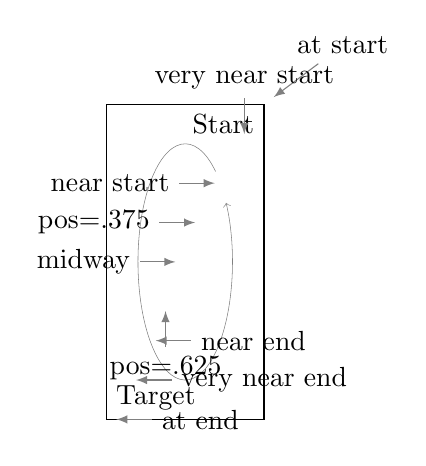
\begin{tikzpicture}[scale=2, every pin edge/.style={latex-, gray}]
\coordinate [label=above right:Target] (A) at (0,0);
\coordinate [label=below left:Start]   (B) at (1,2);
\draw[->, help lines] ([shift=(50:.3 and .75)] .5,1)
  arc[start angle=50, delta angle=340, x radius=.3, y radius=.75];
\draw (B) rectangle (A)
  foreach \pos/\ang in {at start/60, very near start/90, near start/180, pos=.375/180,
                        midway/180, pos=.625/270, near end/0, very near end/0, at end/0}{
    node[pin=\ang:\pos, style/.expanded=\pos]{}};
\end{tikzpicture}
\end{codeexample}

\subsection{Parabola}

For the |parabola| path operator the timer is similar to the |.. controls ..| operator.

The position 0.5 will lie at the |bend|.
\begin{codeexample}[width=.3\linewidth,preamble=\usetikzlibrary{paths.timer}]
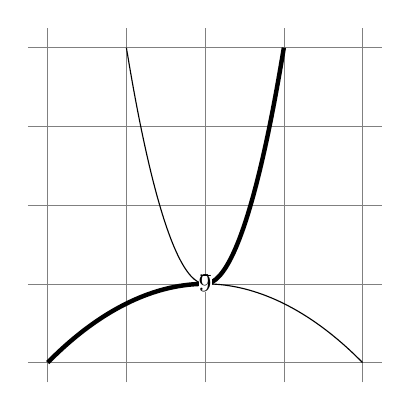
\begin{tikzpicture}
\draw[help lines]  (-2.25, -1.25) grid (2.25, 3.25);
\draw              ( 2,-1) parabola bend (0,0) (-1,3);
\draw[ultra thick] (-2,-1) parabola bend (0,0) ( 1,3)
  foreach \pos in {1,...,4,6,7,...,9}{
    node[
      pos=.\pos, sloped, fill=white, font=\small, inner sep=+0pt
    ] {\pos}
  };
\end{tikzpicture}
\end{codeexample}

If no |bend| is specified half the positions will collapse into one end of the curve.

\begin{codeexample}[width=.3\linewidth,preamble=\usetikzlibrary{paths.timer}]
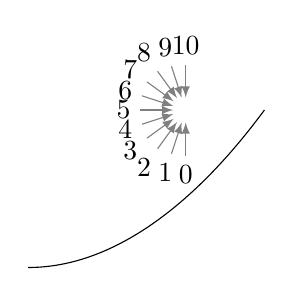
\begin{tikzpicture}[every pin edge/.style={latex-, shorten <=1pt, gray}]
\draw (-2,-2) parabola (1,0)
  foreach \pos in {0, 1, ..., 10} {
    node [pos=\pos/10, pin={[anchor=-18*\pos+90]-18*\pos+270:\pos}]{}
  };
\end{tikzpicture}
\end{codeexample}

\subsection{Sine/Cosine}

The |sin| and |cos| path operators also allow placing of nodes along their paths.

\begin{codeexample}[width=.3\linewidth,preamble=\usetikzlibrary{paths.timer}]
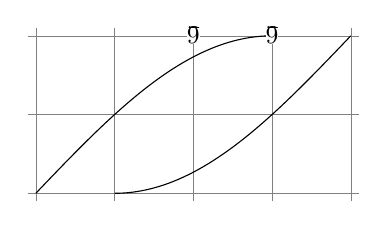
\begin{tikzpicture}[mark nodes on line/.style={insert path={
  foreach \pos in {1, ..., 9} {node[
    sloped, fill=white, font=\small, inner sep=+0pt, pos=\pos/10] {\pos}}}}]
\draw[help lines] (-2.1,-2.1) grid (2.1,0.1);
\draw             (-2,-2) sin (1,0) [mark nodes on line];
\draw[shift=(0:1)](-2,-2) cos (1,0) [mark nodes on line];
\end{tikzpicture}
\end{codeexample}

\endinput
\tikzsetfigurename{patterns.images} % !TeX spellcheck = en_US
% !TeX root = tikz-ext-manual.tex
% Copyright 2022 by Qrrbrbirlbel
%
% This file may be distributed and/or modified
%
% 1. under the LaTeX Project Public License and/or
% 2. under the GNU Free Documentation License.
%
\clearpage
\section{Using Images as a Pattern}
\label{library:patterns.images}

\begin{tikzlibrary}{ext.patterns.images}
  This library allows to use an image to be used as a repeating pattern for a path.
  
  \inspiration{Pattern-Q}{Pattern-A}
\end{tikzlibrary}

With this library arbitrary images (or indeed PDF documents) can be used as
a repeating pattern for the background of a path.

This is a two-step process:
\begin{enumerate}
\item Declaring an image as an ``image-pattern''.
\item Using the ``image-pattern''.
\end{enumerate}

\begin{command}{\pgfsetupimageaspattern\oarg{options}\marg{name}\marg{image}}
\end{command}

\begin{key}{/tikz/image as pattern=\meta{options} (default \{\})}

\begin{codeexample}[preamble=\usetikzlibrary{ext.patterns.images,shapes.geometric}]
\pgfsetupimageaspattern[width=.5cm]{grid}{example-image-1x1}
\tikz \node[star, minimum size=3cm, draw,
  image as pattern={name=grid,options={left, bottom, y=-.5cm, rotate=45}}] {};
\end{codeexample}
\end{key}

\begin{key}{/tikz/image as pattern/name=\meta{name}}
Specifies the name of the ``image-pattern'' to be used.
\end{key}

\begin{stylekey}{/tikz/image as pattern/option}
Options that will be used by the internal |\pgftext|,\indexCommandO{\pgftext}
only keys from |/pgf/text| should be used.\indexKeyO[/pgf/]{text}
\end{stylekey}

\begin{stylekey}{/tikz/image as pattern/options=\meta{style}}
Appends style |/tikz/image as pattern/option|.
\end{stylekey}
\tikzsetfigurename{positioning-plus}
% !TeX spellcheck = en_US
% !TeX root = tikz-ext-manual.tex
% Copyright 2022 by Qrrbrbirlbel
%
% This file may be distributed and/or modified
%
% 1. under the LaTeX Project Public License and/or
% 2. under the GNU Free Documentation License.
%
\clearpage
\section{Positioning Plus}
\label{library:positioning-plus}
\tikzsetnextfilename{posplus}
\begin{tikzlibrary}{ext.positioning-plus}
  With the help of the |positioning|\indexLibrary{positioning} and the |fit|\indexLibrary{fit} library this extends the placement of nodes.
\end{tikzlibrary}

\subsection{Useful corner anchors}
The anchors |corner north east|, |corner north west|, |corner south west| and |corner south east|
are defined as ``generic anchors'', i.\,e. they are defined for all shapes.
This is mostly useful for the placement of circular shapes.
\begin{stylekey}{/tikz/corner above left=\opt{\meta{specification}} (default 0pt)}
  Similar as \referenceKeyandIndexO{above left} of the \tikzname\space library |positioning|
  but uses the |corner north west| anchor.
\end{stylekey}
\begin{stylekey}{/tikz/corner below left=\opt{\meta{specification}} (default 0pt)}
  Similar as \referenceKeyandIndexO{below left} of the \tikzname\space library |positioning|
  but uses the |corner south west| anchor.
\end{stylekey}
\begin{stylekey}{/tikz/corner above right=\opt{\meta{specification}} (default 0pt)}
  Similar as \referenceKeyandIndexO{above right} of the \tikzname\space library |positioning|
  but uses the |corner north east| anchor.
\end{stylekey}
\begin{stylekey}{/tikz/corner below right=\opt{\meta{specification}} (default 0pt)}
  Similar as \referenceKeyandIndexO{below right} of the \tikzname\space library |positioning|
  but uses the |corner south east| anchor.
\end{stylekey}

\begin{codeexample}[width=.6\linewidth,preamble=\usetikzlibrary{ext.positioning-plus}]
\Huge
\begin{tikzpicture}
\node[name=s,shape=circle,shape example]
  {Circle\vrule width 1pt height 2cm};
\foreach \anchor/\placement in {
  north west/above left, north/above, north east/above right,
  west/left, center/above, east/right,
  mid west/right, mid/above, mid east/left,
  base west/left, base/below, base east/right,
  south west/below left, south/below, south east/below right,
  text/left, 10/right, 130/above}
  \draw[shift=(s.\anchor)] plot[mark=x] coordinates{(0,0)}
    node[\placement] {\scriptsize\texttt{(s.\anchor)}};
\draw (s.corner north west) rectangle (s.corner south east);
\foreach \anchor/\placement in {
  corner north west/above left, corner north east/above right,
  corner south west/below left, corner south east/below right}
  \draw[red,shift=(s.\anchor)] plot[mark=x] coordinates{(0,0)}
    node[\placement] {\scriptsize\texttt{(s.\anchor)}};
\end{tikzpicture}
\end{codeexample}

\subsection{Useful placement keys for vertical and horizontal alignment}
\begin{stylekey}{/tikz/north left=\opt{\meta{specification}} (default 0pt)}
  Like \referenceKeyandIndexO{left} but aligns the nodes at their |north| border.
  
  This is basically the same as |left=of reference.north west, anchor=north east|.
  %
\begin{codeexample}[preamble=\usetikzlibrary{ext.positioning-plus}]
\begin{tikzpicture}[nodes=draw]
\node[minimum height=2cm] (a) {};
\node[minimum height=3cm, north right=of a] {};
\end{tikzpicture}
\end{codeexample}
\end{stylekey}
\begin{stylekey}{/tikz/north right=\opt{\meta{specification}} (default 0pt)}
  Like \referenceKeyandIndexO{right} but aligns the nodes at their |north| border.
  
  This is basically the same as |left=of reference.north east, anchor=north west|.
\end{stylekey}
\begin{stylekey}{/tikz/south left=\opt{\meta{specification}} (default 0pt)}
  Like \referenceKeyandIndexO{left} but aligns the nodes at their |south| border.
  
  This is basically the same as |left=of reference.south west, anchor=south east|.
\end{stylekey}
\begin{stylekey}{/tikz/south right=\opt{\meta{specification}} (default 0pt)}
  Like \referenceKeyandIndexO{right} but aligns the nodes at their |south| border.
  
  This is basically the same as |left=of reference.south east, anchor=south west|.
\end{stylekey}
\begin{stylekey}{/tikz/west above=\opt{\meta{specification}} (default 0pt)}
  Like \referenceKeyandIndexO{above} but aligns the nodes at their |west| border.
  
  This is basically the same as |left=of reference.north west, anchor=south west|.
\end{stylekey}
\begin{stylekey}{/tikz/west below=\opt{\meta{specification}} (default 0pt)}
  Like \referenceKeyandIndexO{below} but aligns the nodes at their |west| border.
  
  This is basically the same as |left=of reference.south west, anchor=north west|.
\end{stylekey}
\begin{stylekey}{/tikz/east above=\opt{\meta{specification}} (default 0pt)}
  Like \referenceKeyandIndexO{above} but aligns the nodes at their |east| border.
  
  This is basically the same as |left=of reference.north east, anchor=south east|.
\end{stylekey}
\begin{stylekey}{/tikz/east below=\opt{\meta{specification}} (default 0pt)}
  Like \referenceKeyandIndexO{below} but aligns the nodes at their |east| border.
  
  This is basically the same as |left=of reference.south east, anchor=north east|.
\end{stylekey}

The same exist for the recently introduces corner anchors, too.
\begin{stylekey}{/tikz/corner north left=\opt{\meta{specification}} (default 0pt)}
  The same as |/tikz/north left| but uses the new corner anchors.
\end{stylekey}
\begin{stylekey}{/tikz/corner north right=\opt{\meta{specification}} (default 0pt)}
  The same as |/tikz/north right| but uses the new corner anchors.
\end{stylekey}
\begin{stylekey}{/tikz/corner south left=\opt{\meta{specification}} (default 0pt)}
  The same as |/tikz/south left| but uses the new corner anchors.
\end{stylekey}
\begin{stylekey}{/tikz/corner south right=\opt{\meta{specification}} (default 0pt)}
  The same as |/tikz/south right| but uses the new corner anchors.
\end{stylekey}
\begin{stylekey}{/tikz/corner west above=\opt{\meta{specification}} (default 0pt)}
  The same as |/tikz/west above| but uses the new corner anchors.
\end{stylekey}
\begin{stylekey}{/tikz/corner west below=\opt{\meta{specification}} (default 0pt)}
  The same as |/tikz/west below| but uses the new corner anchors.
\end{stylekey}
\begin{stylekey}{/tikz/corner east above=\opt{\meta{specification}} (default 0pt)}
  The same as |/tikz/east above| but uses the new corner anchors.
\end{stylekey}
\begin{stylekey}{/tikz/corner east below=\opt{\meta{specification}} (default 0pt)}
  The same as |/tikz/east below| but uses the new corner anchors.
\end{stylekey}

While the \meta{specification} of all these keys still accept the same form as with \tikzname,
the |ext.positioning-plus| library extends this even more.

The specification after |of| can contain a list of coordinates
(like the |fit| key of the |fit| library).
This means that the new node will be placed in relation to a rectangular bounding box
that fits around all this nodes in the list.

If this list is prefixed with \verb!|!, |-| or |+|,
the new node will also have the same height (\verb!|!),
the same width (|-|) or both as this bounding box.

\begin{codeexample}[preamble=\usetikzlibrary{ext.positioning-plus}]
\begin{tikzpicture}[nodes=draw]
\node                     (A) {A};
\node[below=of A]         (BCD) {BCD};
\node[right=of |(A)(BCD)] (c) {};
\node[below=.5:of -(A)(BCD)] (d) {};
\draw[help lines] (BCD.south west) -- (c.south east)
                  (BCD.north east) -- (d.south east);
\end{tikzpicture}
\end{codeexample}

This functionality is also available without the placement:
\begin{stylekey}{/tikz/fit bounding box=\meta{list of coordinates}}
  Creates a rectangular node with the name |fit bounding box| that encompasses
  the \meta{list of coordinates}.
\end{stylekey}
\begin{stylekey}{/tikz/span vertical=\meta{list of coordinates}}
  Creates a rectangular node with the name |fit bounding box| that encompasses
  the \meta{list of coordinates} \emph{and} sets the \referenceKeyandIndexO[/pgf]{minimum height} to
  the height of this bounding box.
\end{stylekey}
\begin{stylekey}{/tikz/span horizontal=\meta{list of coordinates}}
  Creates a rectangular node with the name |fit bounding box| that encompasses
  the \meta{list of coordinates} \emph{and} sets the \referenceKeyandIndexO[/pgf]{minimum width} to
  the width of this bounding box.
\end{stylekey}
\begin{stylekey}{/tikz/span=\meta{list of coordinates}}
  Is a combination of |/tikz/span vertical| and |/tikz/span horizontal|.
\end{stylekey}

As you maybe noticed in the example above, the \meta{specification} also allows a prefix
delimited by |:| which the |node distance| will be multiplied to with for the placement.%
\footnote{This is probably more useful when \referenceKeyandIndexO{on grid} is used.}

\endinput
\tikzsetfigurename{scalepicture}
% !TeX spellcheck = en_US
% !TeX root = tikz-ext-manual.tex
% Copyright 2022 by Qrrbrbirlbel
%
% This file may be distributed and/or modified
%
% 1. under the LaTeX Project Public License and/or
% 2. under the GNU Free Documentation License.
%
\clearpage
\section{Scaling Pictures to a Specific Size}
\label{library:scalepicture}

\begin{tikzlibrary}{ext.scalepicture}
  This library scales \tikzname\ pictures to a specific width or height
  by scaling the whole picture.
\end{tikzlibrary}

\begin{multicols}{2}
If one of the keys below are used on a \tikzname\ picture, i.\,e.
as an option |\tikzpicture| or \texttt{\textbackslash begin\{tikzpicture\}}
the size of the picture\footnote{This is the size of the pseudo-node \texttt{current bounding box}.}
will be measured and written to the \filetype{aux} file
so that it will be available at the next compilation run
and an appropriate scaling for the picture can be installed.

\begin{command}{\tikzextpicturewidth}
  Returns the last measured width of the picture.
  
  This will expand to |0pt| if the picture hasn't been measured before.
\end{command}
\begin{command}{\tikzextpictureheight}
  Returns the last measured height of the picture.
  
  This will expand to |0pt| if the picture hasn't been measured before.
\end{command}

\subsection{Keeping the aspect ratio}
The following \emph{unstarred} keys do not change the aspect ratio of the picture.

\begin{key}{/tikz/picture width=\meta{dimension}}
  Scales the picture so that the width of the picture will be \meta{dimension}.
  This will keep the aspect ratio the same.
\end{key}

\begin{key}{/tikz/minimum picture width=\meta{dimension}}
  As above but will not change the size of the picture
  if its width is greater than \meta{dimension}.
\end{key}

\begin{key}{/tikz/maximum picture width=\meta{dimension}}
  As above but will not change the size of the picture
  if its width is less than \meta{dimension}.
\end{key}

\begin{key}{/tikz/picture height=\meta{dimension}}
  Scales the picture so that the height of the picture will be \meta{dimension}.
  This will keep the aspect ratio the same.
\end{key}

\begin{key}{/tikz/minimum picture height=\meta{dimension}}
  As above but will not change the size of the picture
  if its height is greater than \meta{dimension}.
\end{key}

\begin{key}{/tikz/maximum picture height=\meta{dimension}}
  As above but will not change the size of the picture
  if its height is less than \meta{dimension}.
\end{key}

\begin{key}{/tikz/minimum picture size=\marg{width}\marg{height}}
  Scales the picture so that its height will be at least \meta{width}
  and its height will be at least \meta{height}.
\end{key}

\begin{key}{/tikz/maximum picture size=\marg{width}\marg{height}}
  Scales the picture so that its height will be at most \meta{width}
  and its height will be at most \meta{height}.
\end{key}

\subsection{Changing the aspect ratio.}
The following \emph{starred} keys do change the aspect ratio.
\begin{key}{/tikz/picture width*=\meta{dimension}}
\end{key}

\begin{key}{/tikz/picture height*=\meta{dimension}}
\end{key}

\begin{key}{/tikz/picture size*=\meta{dimension}}
\end{key}
\end{multicols}
\tikzsetfigurename{topaths}
% !TeX root = tikz-ext-manual.tex
% !TeX spellcheck = en_US
% Copyright 2022 by Qrrbrbirlbel
%
% This file may be distributed and/or modified
%
% 1. under the LaTeX Project Public License and/or
% 2. under the GNU Free Documentation License.
%

\section{Arcs through Three Points}
\label{library:topaths.arcthrough}
\begin{tikzlibrary}{ext.topaths.arcthrough}
  This library allows to use an arc defined by three points.
\end{tikzlibrary}

\begin{codeexample}[width=10cm,preamble=\usetikzlibrary{ext.topaths.arcthrough}]
\begin{tikzpicture}
\coordinate[label=above right:$A$] (A) at ( 3, 1);
\coordinate[label=above:$B$]       (B) at ( 1, 2);
\coordinate[label=below left:$C$]  (C) at (-2,-2);

\draw[ultra thick, draw=green, fill=green!50]
  (B) to[arc through={clockwise,(A)}] (C) 
  -- (arc through center) -- cycle;
\draw[ultra thick, draw=blue, fill=blue!50]
  (B) to[arc through=(A)]             (C)
  -- (arc through center) -- cycle;

\foreach \p in {A,B,C, arc through center} \fill[red] (\p) circle[radius=2pt];
\end{tikzpicture}
\end{codeexample}

This can only by used for circles in the |canvas| coordinate system.

\begin{multicols}{2}
\begin{key}{/tikz/arc through/through=\meta{coordinate} (initially {(0,0)})}
  The coordinate on the circle that defines~-- together with the
  starting and target point~-- a circle.
\end{key}

\begin{key}{/tikz/arc through/center suffix=\meta{suffix} (initially {})}
  The |arc through| will define a coordinate named |arc through center|\meta{suffix}
  so that it can be referenced later.
\end{key}

\begin{key}{/tikz/arc through/clockwise}
  The resulting arc will go clockwise from the starting point to the target point.
  This will not necessarily go through the |through| point.
\end{key}

\begin{key}{/tikz/arc through/counter clockwise}
  The resulting arc will go counter clockwise from the starting point to the target point.
  This will not necessarily go through the |through| point.
\end{key}

\begin{key}{/tikz/arc through=\meta{key-value}}
  This key should be used with |to|\indexPathOperationO{to} or |edge|\indexPathOperationO{edge}.
  A parameter other than |center suffix|, |clockwise| or |counter clockwise| will
  be assumed to be the |through| coordinate.
\end{key}
\end{multicols}
\endinput
% !TeX root = tikz-ext-manual.tex
% !TeX spellcheck = en_US
% Copyright 2023 by Qrrbrbirlbel
%
% This file may be distributed and/or modified
%
% 1. under the LaTeX Project Public License and/or
% 2. under the GNU Free Documentation License.
%

\section{Autobending}
\label{library:topaths.autobend}
\begin{tikzlibrary}{ext.topaths.autobend}
  This library provides various bended |to| paths
  that bend in the specified direction.
  
  \inspiration{AutoBend-Q}{AutoBend-A}
\end{tikzlibrary}

The keys \referenceKeyandIndexO{bend left}
and \referenceKeyandIndexO{bend left} from \tikzname\ 
bend the requested curve in relation of the connecting
coordinates/nodes.

The keys provided by this library bend the curve in the direction relative
to the paper (north, south, west and east) or relative to the current
coordinate system (up, down, left and right).

\begin{key}{/tikz/ext/autobend north=\meta{angle} (default \normalfont last value)}
  Works like the |bend left| and |bend right| options
  but bends the curve to the top of the page (i.\,e. it ignores the current transformation).
\end{key}
\begin{key}{/tikz/ext/autobend south=\meta{angle} (default \normalfont last value)}
  Works like |autobend north| but bends the curve to the bottom of the page.
\end{key}
\begin{key}{/tikz/ext/autobend west=\meta{angle} (default \normalfont last value)}
  Works like |autobend north| but bends the curve to the left of the page.
\end{key}
\begin{key}{/tikz/ext/autobend east=\meta{angle} (default \normalfont last value)}
  Works like |autobend north| but bends the curve to the right of the page.
\end{key}

\begin{key}{/tikz/ext/autobend up=\meta{angle} (default \normalfont last value)}
  Works like the |bend left| and |bend right| options
  but bends the curve upwards (i.\,e. it observes the current transformation).
\end{key}
\begin{key}{/tikz/ext/autobend down=\meta{angle} (default \normalfont last value)}
  Works like |autobend up| but bends the curve downwards.
\end{key}
\begin{key}{/tikz/ext/autobend left=\meta{angle} (default \normalfont last value)}
  Works like |autobend up| but bends the curve leftwards.
\end{key}
\begin{key}{/tikz/ext/autobend right=\meta{angle} (default \normalfont last value)}
  Works like |autobend up| but bends the curve rightwards.
\end{key}

\begin{codeexample}[preamble=\usetikzlibrary{arrows.meta, ext.topaths.autobend},width=6cm]
\begin{tikzpicture}[
  every path/.append style=-Latex,
  pics/cs/.style={
    /tikz/transform shape,
    code={\draw[help lines, Latex-Latex] (up:1) |- (right:1);}
  },
  nodes={sloped, fill=white, inner ysep=+.1em, fill opacity=.8, text opacity=1, scale=.5}]
\foreach[count=\i] \c/\d in {black/north, red/south,
                             green!50!black/west, yellow!50!black/east}
  \draw[\c] (0,0) pic {cs} to[ext/autobend \d=\i0] node{\d} +(45:3);
\foreach[count=\i] \c/\d in {black/north, red/south,
                             green!50!black/west, yellow!50!black/east}
  \draw[shift=(right:2), rotate=180, \c]
          (45:-3) pic {cs} to[ext/autobend \d=\i0] node{\d} (0,0);

\tikzset{shift=(down:2.5)}
\foreach[count=\i] \c/\d in {black/up, red/down,
                             green!50!black/left, yellow!50!black/right}
  \draw[\c] (0,0) pic {cs} to[ext/autobend \d=\i0] node{\d} +(45:3);
\foreach[count=\i] \c/\d in {black/up, red/down,
                             green!50!black/left, yellow!50!black/right}
  \draw[shift=(right:2), rotate=180, \c]
          (45:-3) pic {cs} to[ext/autobend \d=\i0] node{\d} (0,0);
\end{tikzpicture}
\end{codeexample}
\tikzsetfigurename{trans}
% Copyright 2022 by Qrrbrbirlbel
%
% This file may be distributed and/or modified
%
% 1. under the LaTeX Project Public License and/or
% 2. under the GNU Free Documentation License.
%

\clearpage
\section{Mirror, Mirror on the Wall}
\label{library:mirror}

\begin{tikzlibrary}{ext.transformations.mirror}
  This library adds more transformations to \tikzname.
\end{tikzlibrary}

As explained in section~\ref{pgflibrary:transformations}, they are two approaches to setting a mirror transformation.
As with the commands in PGF, we'll be using lowercase |m| for the ``Spiegelungsmatrix'' and uppercase |M| for the built-in approach.

\subsection{Using the ``Spiegelungsmatrix''}

\begin{codeexample}[width=.4\linewidth,preamble=\usetikzlibrary{shapes.geometric,ext.transformations.mirror}]
\begin{tikzpicture}[line join=round, thick, reg poly/.style={
  shape=regular polygon, regular polygon sides={#1}}]
\node[reg poly=5, minimum size=+2cm, draw, very thick] (a) {};
\foreach \i[evaluate={\col=(\i-1)/.04}] in {1,...,5}
  \node [mirror=(a.corner \i)--(a.side \i), transform shape,
         reg poly=5, minimum size=+2cm, draw=red!\col!blue] {};
\end{tikzpicture}
\end{codeexample}

\begin{key}{/tikz/xmirror=\meta{value or coordinate}}
  Sets up a transformation that mirrors along a horizontal line that goes through point $(\text{\meta{value}}, 0)$ or \meta{coordinate}.

\begin{codeexample}[preamble=\usetikzlibrary{ext.transformations.mirror}]
\begin{tikzpicture}
\draw[help lines] (-0.25, -.25) grid (3.25, 1.25);
\draw[-latex] (0,0) .. controls (.5,1) .. (1,1);

\draw[dashed] (1.5, -.25) coordinate (m) -- (1.5, 1.25);
\draw[xmirror=(m),-latex] (0,0) .. controls (.5,1) .. (1,1);
\end{tikzpicture}
\end{codeexample}
\end{key}

\begin{key}{/tikz/ymirror=\meta{value or coordinate}}
  Sets up a transformation that mirrors along a vertical line that goes through point $(0, \text{\meta{value}})$ or \meta{coordinate}.
\end{key}


\begin{key}{/tikz/mirror x=\meta{coordinate}}
  Similar to |/tikz/xmirror|, this however uses the |xyz| coordinate system instead of the |canvas| system.
\begin{codeexample}[preamble=\usetikzlibrary{ext.transformations.mirror}]
\begin{tikzpicture}[x=.5cm, y=(45:1cm)]

\draw[-latex] (0,0) .. controls (.5,1) .. (1,1);

\draw[dashed] (1.5, -.25) coordinate (m) -- (1.5, 1.25);

\draw[ xmirror=(m), -latex, red, dotted] (0,0) .. controls (.5,1) .. (1,1);
\draw[mirror x=(m), -latex]              (0,0) .. controls (.5,1) .. (1,1);
\end{tikzpicture}
\end{codeexample}
\end{key}

\begin{key}{/tikz/mirror y=\meta{coordinate}}
  Similar to |/tikz/ymirror|, this however uses the |xyz| coordinate system instead of the |canvas| system.
\end{key}


\begin{key}{/tikz/mirror=\meta{point A}|--|\meta{point B}}
  Sets up a transformation that mirrors along a line that goes through \meta{point A} and \meta{point B}.
  
  When only \meta{point A} is given that line goes through \meta{point A} and the origin.
\end{key}

\subsection{Using built-in transformations}

\begin{codeexample}[width=.4\linewidth,preamble=\usetikzlibrary{shapes.geometric,ext.transformations.mirror}]
\begin{tikzpicture}[line join=round, thick, reg poly/.style={
  shape=regular polygon, regular polygon sides={#1}}]
\node[reg poly=5, minimum size=+2cm, draw, very thick] (a) {};
\foreach \i[evaluate={\col=(\i-1)/.04}] in {1,...,5}
  \node [Mirror=(a.corner \i)--(a.side \i), transform shape,
         reg poly=5, minimum size=+2cm, draw=red!\col!blue] {};
\end{tikzpicture}
\end{codeexample}

\begin{key}{/tikz/xMirror=\meta{value or coordinate}}
  Sets up a transformation that mirrors along a horizontal line that goes through point $(\text{\meta{value}}, 0)$ or \meta{coordinate}.

\begin{codeexample}[preamble=\usetikzlibrary{ext.transformations.mirror}]
\begin{tikzpicture}
\draw[help lines] (-0.25, -.25) grid (3.25, 1.25);
\draw[-latex] (0,0) .. controls (.5,1) .. (1,1);

\draw[dashed] (1.5, -.25) coordinate (m) -- (1.5, 1.25);
\draw[xMirror=(m),-latex] (0,0) .. controls (.5,1) .. (1,1);
\end{tikzpicture}
\end{codeexample}
\end{key}

\begin{key}{/tikz/yMirror=\meta{value or coordinate}}
  Sets up a transformation that mirrors along a vertical line that goes through point $(0, \text{\meta{value}})$ or \meta{coordinate}.
\end{key}


\begin{key}{/tikz/Mirror x=\meta{coordinate}}
  Similar to |/tikz/xMirror|, this however uses the |xyz| coordinate system instead of the |canvas| system.
\begin{codeexample}[preamble=\usetikzlibrary{ext.transformations.mirror}]
\begin{tikzpicture}[x=.5cm, y=(45:1cm)]

\draw[-latex] (0,0) .. controls (.5,1) .. (1,1);

\draw[dashed] (1.5, -.25) coordinate (m) -- (1.5, 1.25);

\draw[ xMirror=(m), -latex, red, dotted] (0,0) .. controls (.5,1) .. (1,1);
\draw[Mirror x=(m), -latex]              (0,0) .. controls (.5,1) .. (1,1);
\end{tikzpicture}
\end{codeexample}
\end{key}

\begin{key}{/tikz/Mirror y=\meta{coordinate}}
  Similar to |/tikz/yMirror|, this however uses the |xyz| coordinate system instead of the |canvas| system.
\end{key}


\begin{key}{/tikz/Mirror=\meta{point A}\opt{|--|\meta{point B}}}
  Sets up a transformation that mirrors along a line that goes through \meta{point A} and \meta{point B}.
  
  When only \meta{point A} is given that line goes through \meta{point A} and the origin.
\end{key}

\endinput
%
\part{\pgfname\space Libraries}
\label{part:pgf}
These libraries (should) work with both \pgfname\space and \tikzname.

\begin{center}\tikzsetnextfilename{main-graph}
\begin{codeexample}[width=10cm,preamble=%
  \usetikzlibrary{graphs,graphdrawing,ext.misc} \usegdlibrary{force}]
\tikzset{
  mynode/.style={
    circle, minimum size=10mm, draw, densely dashdotted, thick,
    decide color/.expand once=#1},
  decide color/.style 2 args={
    /utils/ext/if=c#1
      {/utils/ext/ifnum={#2<5}{bluelight}{bluedark}}
      {/utils/ext/ifnum={#2<8}{light}{dark}}},
  light/.style={fill=gray!20},  bluelight/.style={fill=blue!10},
  dark/.style ={fill=gray!60},  bluedark/.style ={fill=blue!30}}
\tikz\graph[
  spring electrical layout, vertical=c2 to p13,
  node distance=1.5cm, typeset=$n_{\tikzgraphnodetext}$,
  nodes={mynode=\tikzgraphnodetext}] {
  % outer ring
  c2 -- {p1, p11, p6};
    p1 -- {p8, c6, p11};
      p8 -- {p3, p10, c6};
       p3 -- {p13, p15, p10};
         p13 -- {p15, c7};
           c7  -- {c3, c4, p15};
           c3  -- {p14, c4};
           p14 -- {p7, c4};
         p7 -- {p9, p2, c4};
       p9 -- {c5, p12, p2};
     c5 -- {c1, p4, p12};
   c1 -- {p6, p4};
  p6 -- {p11, p4};
  % inner ring
  p11 -- {c6, p12, p4};
  p5 -- {c6 -- {p10, p12}, p10 -- p15, p15 -- c4, c4 -- p2, p2 -- p12, p12 -- p4};
};
\end{codeexample}
\end{center}

\tikzsetfigurename{PGF.arrows}% !TeX spellcheck = en_US
% !TeX root = tikz-ext-manual.tex
% Copyright 2023 by Qrrbrbirlbel
%
% This file may be distributed and/or modified
%
% 1. under the LaTeX Project Public License and/or
% 2. under the GNU Free Documentation License.
%

\section{Arrow Tips}
\label{pgflibrary:arrows}
\tikzset{external/export/.try=false}%
\begin{pgflibrary}{ext.arrows}
  This library adds arrows to \pgfname/\tikzname.
  
  \inspiration{ArrowLoop-Q,ArrowHug-Q,ArrowUntipped1-Q,ArrowUntipped2-Q}
              {ArrowLoop-A,ArrowHug-A,ArrowUntipped1-A,ArrowUntipped2-A}
\end{pgflibrary}
\begin{multicols}{2}
The arrow tips of the \referenceLibraryandIndexO{arrows.meta} library always
just touch the end of original line -- which is usually
what you want.

But for some arrow tips (and when they lie along a path) it makes sense
that these tips shoot a bit over the end of the line.
This is why these arrow tips exist.
They can be categorized into three groups:
\begin{enumerate}
\item Centered
\item Untipped
\item Overtipped\footnote{The Overtipped arrow tips aren't yet implemented.}
\end{enumerate}
Not all original arrow tips got all variants.
For a summary, refer to table on the right side.
As with the original tips of the \referenceLibraryandIndexO{arrows.meta} library
these can be organized in the following categories.
\newcolumn
\begin{center}
\newcommand*\tip[2][]{%
  \tikzset{external/export/.try=false}%
  \tikz[arrows={ext_#2 \arrowtiprow[reversed] - \arrowtiprow[sep] . ext_#2 \arrowtiprow[]}, baseline=+-.5ex,
    trim left=+-3mm, trim right=+13mm]
    \draw[line width=+.5mm, postaction={draw, gray, thin,-}] (0,0) -- + (right:1);%
}%
\def\tiprow#1 &{#1\gdef\arrowtiprow{#1} &}%
\def\Tiprow#1 &{\quad#1\gdef\arrowtiprow{#1} &}%
%\centering
%\caption{Variants of the original \texttt{arrows.meta} arrow tips.
%  For each example, the order is 1. reversed variant, 2. original, 3. variant.
%  They gray line shows where the path actually ends.
%}\label{tab:tips}
\begin{tabular}{ll ccc}
  \toprule
  Group        & Original                   & Centered       &    Untipped    & Overtipped \\ \midrule
  Barbed       & \tiprow Arc Barb           & \tip{Centered} & \tip{Untipped} &     --     \\
               & \Tiprow Parenthesis        & \tip{Centered} & \tip{Untipped} &     --     \\
               & \tiprow Hooks              & \tip{Centered} &       --       &     --     \\
               & \tiprow Straight Barb      & \tip{Centered} &       --       &     --     \\
               & \tiprow Tee Barb           & \tip{Centered} & \tip{Untipped} &     --     \\
               & \Tiprow Bar                & \tip{Centered} & \tip{Untipped} &     --     \\
               & \Tiprow Bracket            & \tip{Centered} & \tip{Untipped} &     --     \\ \midrule
%  Mathematical & Classical TikZ Rightarrow  & --             &       --       &     --     \\
%               & Computer Modern Rightarrow & --             &       --       &     --     \\
%               & \quad To                   & --             &       --       &     --     \\
%               & Implies                    & --             &       --       &     --     \\ \midrule
  Geometric    & \tiprow Circle             & \tip{Centered} & \tip{Untipped} &     --     \\
               & \Tiprow Ellipse            & \tip{Centered} & \tip{Untipped} &     --     \\
               & \tiprow Kite               & \tip{Centered} &       --       &     --     \\
               & \Tiprow Diamond            & \tip{Centered} &       --       &     --     \\
               & \Tiprow Turned Square      & \tip{Centered} &       --       &     --     \\
               & \tiprow LaTeX              & --             &       --       &     --     \\
               & \tiprow Square             & \tip{Centered} &       --       &     --     \\
               & \Tiprow Rectangle          & \tip{Centered} &       --       &     --     \\
               & \tiprow Stealth            & \tip{Centered} &       --       &     --     \\
               & \Tiprow Triangle           & \tip{Centered} &       --       &     --     \\ \midrule
%  Caps         &                            & --             &       --       &     --     \\
  Rays         & \tiprow Rays               & \tip{Centered} &       --       &     --     \\ \bottomrule
\end{tabular}
\end{center}
\newcolumn

\subsection{Centered}
\subsubsection{Barbed Arrow Tips}
\begin{arrowtipsimple}{ext\textunderscore Centered Arc Barb}\tipcompat
    This is a variant of the \referenceArrowtipandIndexO{Arc Barb} tip.
    The center of the arc lies on the original end of the path.
\end{arrowtipsimple}

\begin{arrowtipsimple}{ext\textunderscore Centered Bar}\tipcompat
    A variant of the simple \referenceArrowtipandIndexO{Bar} tip.
    This is a simple instance of |ext_Centered Tee Barb| for length zero.
    
    The middle of the line will lie on original end of the path.
\end{arrowtipsimple}

\begin{arrowtipsimple}{ext\textunderscore Centered Bracket}\tipcompat
    This is a variant of the \referenceArrowtipandIndexO{Bracket} tip and
    therefore an instance of the |ext_Centered Tee Barb| arrow tip that results in something
    resembling a bracket.
    
    The middle of the vertical part will lie on the original end of the path.
\end{arrowtipsimple}

\begin{arrowtipsimple}{ext\textunderscore Centered Hooks}\tipcompat
    A variant of the \referenceArrowtipandIndexO{Hooks} tip.
    The starting point of the hooks will lie on the original end of the path.
\end{arrowtipsimple}

\begin{arrowtipsimple}{ext\textunderscore Centered Parenthesis}\tipcompat
    This is a variant of the \referenceArrowtipandIndexO{Parenthesis} tip and
    thus an instance of the |ext_Centered Arc Barb| arrow tip.
\end{arrowtipsimple}

\begin{arrowtipsimple}{ext\textunderscore Centered Straight Barb}\tipcompat
    A variant of the \referenceArrowtipandIndexO{Straight Barb} tip.
\end{arrowtipsimple}

\begin{arrowtipsimple}{ext\textunderscore Centered Tee Barb}\tipcompat
    A variant of the \referenceArrowtipandIndexO{Tee Barb} tip.
    
    The middle of the vertical part will lie on the original end of the path.
\end{arrowtipsimple}

\subsubsection{Geometric Arrow Tips}
\begin{arrowtipsimple}{ext\textunderscore Centered Circle}\tipcompat
    A variant of the \referenceArrowtipandIndexO{Circle} tip.
    The center of the circle will lie on the original end of the path.
\end{arrowtipsimple}

\begin{arrowtipsimple}{ext\textunderscore Centered Diamond}\tipcompat
    This is a variant of the \referenceArrowtipandIndexO{Diamond} tip and
    thus an instance of |ext_Centered Kite| where the length is larger than the width.
\end{arrowtipsimple}

\begin{arrowtipsimple}{ext\textunderscore Centered Ellipse}\tipcompat
    This is a variant of the \referenceArrowtipandIndexO{Ellipse} tip
    and thus another name for the |ext_Centered Circle| tip
    that is twice as wide as high.
\end{arrowtipsimple}

\begin{arrowtipsimple}{ext\textunderscore Centered Kite}\tipcompat
    A variant of the \referenceArrowtipandIndexO{Kite} tip.
    
    The widest part will lie on the original end of the path.
\end{arrowtipsimple}

\begin{arrowtipsimple}{ext\textunderscore Centered Rectangle}\tipcompat
    A variant of the \referenceArrowtipandIndexO{Rectangle} tip.
    By default, it is twice as long as high.
\end{arrowtipsimple}

\begin{arrowtipsimple}{ext\textunderscore Centered Square}\tipcompat
    A variant of the \referenceArrowtipandIndexO{Square} tip.
\end{arrowtipsimple}

\begin{arrowtipsimple}{ext\textunderscore Centered Stealth}\tipcompat
    This is a variant of the \referenceArrowtipandIndexO{Stealth} tip.
    
    The weighted center will lie at the original end of the path.
\end{arrowtipsimple}

\begin{arrowtipsimple}{ext\textunderscore Centered Triangle}\tipcompat
    This is a variant of the \referenceArrowtipandIndexO{Triangle} tip and
    thus an instance of the |ext_Centered Kite| tip with zero inset.
\end{arrowtipsimple}

\begin{arrowtipsimple}{ext\textunderscore Centered Turned Square}\tipcompat
    This is a variant of the \referenceArrowtipandIndexO{Turned Square} tip and
    thus an instance of the |ext_Centered Kite| tip with identical width and height and mid-inset.
\end{arrowtipsimple}

\subsubsection{Special Arrow Tips}
\begin{arrowtipsimple}{ext\textunderscore Centered Rays}\tipcompat
    A variant of the \referenceArrowtipandIndexO{Rays} tip.
    The origin of the rays will lie on the original end of the path.
\end{arrowtipsimple}

\subsection{Untipped}
\subsubsection{Barbed Arrow Tips}
\begin{arrowtipsimple}{ext\textunderscore Centered Arc Barb}\tipcompat
    This is a variant of the \referenceArrowtipandIndexO{Arc Barb} tip.
    The arrow tip will protrude half its line width over the original end of the path.
\end{arrowtipsimple}

\begin{arrowtipsimple}{ext\textunderscore Untipped Bar}\tipcompat
    A variant of the simple \referenceArrowtipandIndexO{Bar} tip.
    This is a simple instance of |ext_Untipped Tee Barb| for length zero.
    
    The middle of the line will lie on original end of the path.
\end{arrowtipsimple}

\begin{arrowtipsimple}{ext\textunderscore Untipped Bracket}\tipcompat
    This is a variant of the \referenceArrowtipandIndexO{Bracket} tip and
    therefore an instance of the |ext_Untipped Tee Barb| arrow tip that results in something
    resembling a bracket.
    
    The arrow tip will protrude half its line width over the original end of the path.
\end{arrowtipsimple}

\begin{arrowtipsimple}{ext\textunderscore Untipped Parenthesis}\tipcompat
    This is a variant of the \referenceArrowtipandIndexO{Parenthesis} tip and
    thus an instance of the |ext_Untipped Arc Barb| arrow tip.
\end{arrowtipsimple}

\begin{arrowtipsimple}{ext\textunderscore Untipped Tee Barb}\tipcompat
    A variant of the \referenceArrowtipandIndexO{Tee Barb} tip.
    
    The middle of the vertical part will lie on the original end of the path.
\end{arrowtipsimple}

\subsubsection{Geometric Arrow Tips}
\begin{arrowtipsimple}{ext\textunderscore Untipped Circle}\tipcompat
    A variant of the \referenceArrowtipandIndexO{Circle} tip.
    This tip will protrude half its line width over the original end of the path.
\end{arrowtipsimple}

\begin{arrowtipsimple}{ext\textunderscore Untipped Ellipse}\tipcompat
    This is a variant of the \referenceArrowtipandIndexO{Ellipse} tip
    and thus another name for the |ext_Untipped Circle| tip
    that is twice as wide as high.
\end{arrowtipsimple}

\newcolumn
\subsection{Original Arrow Tips}
\begin{arrowtipsimple}{ext\textunderscore Hug Cap}\tipcompat
This arrow tips will hug a circle that would touch the end of the path.

Use the \referenceKeyandIndexO[/pgf/arrow keys/]{length} key to set up the radius of that circle.

\begin{codeexample}[preamble=\usepgflibrary{ext.arrows}]
\begin{tikzpicture}[
  dot/.style 2 args={
    shape=circle, outer sep=+0pt, fill={#1}, minimum size={#2}}]
\node[dot={red} {2cm}] (A)           {};
\node[dot={blue}{3cm}] (B) at (6,0) {};
\draw[
  line width=1.5cm,
  arrows={ext_Hug Cap[length=1cm]-ext_Hug Cap[length=1.5cm]}
] (A) to[out=45, in=180] (B);
\end{tikzpicture}
\end{codeexample}
\end{arrowtipsimple}

\makeatletter
\newcommand*\extus{%
  \ifx\path\tikz@command@path
    ext_%
  \else
    ext\textunderscore
  \fi
}
\makeatother
\begin{arrowtip}{\extus Loop}{\tipCompat{Loop}
  This arrow tip attaches a one-sided loop to the end of the line.
  The |length| refers to the length of the whole tip while the |inset|
  specifies the radius of the three rounded corners.
  The width of the tip is twice the |length| (but can't specified independently).
}{length=1.5cm,inset=3.5mm}{length=1.5cm,radius=3.5mm/1.5cm}
    \begin{arrowexamples}
        \arrowexample[]
        \arrowexampledup[sep]
        \arrowexampledupdot[sep]
        \arrowexample[open]
        \arrowexample[open, swap]
        \arrowexample[length=5pt,inset=0pt]
        \arrowexample[reversed]
        \arrowexample[slant=.3]
        \arrowexample[red]
    \end{arrowexamples}
    %
    The following options have no effect: |harpoon|, |round|, |line width|.

    On |double| lines, the arrow tip will not look correct.
\end{arrowtip}
\end{multicols}
\tikzset{external/export/.try=true}%
\endinput

\tikzsetfigurename{PGF.trans}% !TeX spellcheck = en_US
% !TeX root = tikz-ext-manual.tex
% Copyright 2022 by Qrrbrbirlbel
%
% This file may be distributed and/or modified
%
% 1. under the LaTeX Project Public License and/or
% 2. under the GNU Free Documentation License.
%

\section{Transformations: Mirroring}
\label{pgflibrary:transformations}

\begin{purepgflibrary}{ext.transformations.mirror}
  This library adds mirror transformations to \pgfname.
\end{purepgflibrary}

Two approaches to mirror transformation exist:
\begin{enumerate}
\item Using the reflection matrix (see left column).

  This depends on |\pgfpointnormalised|\indexCommandO\pgfpointnormalised which involves
  the sine\indexMathFunctionO{sin} and the cosine\indexMathFunctionO{cos} functions of \pgfname math.

\item Using built-in transformations (see right column).

  This depends on |\pgfmathanglebetweenpoints|\indexCommandO\pgfmathanglebetweenpoints which
  involves the arctangent (|atan2|\indexMathFunctionO{atan2}) function of \pgfname math.
\end{enumerate}

Which one is better? I don't know.
Choose one you're comfortable with.

\begin{paracol}{2}

\subsection{Using the reflection matrix}

The following commands use the reflection matrix that sets the transformation matrix following
\begin{equation*}
  A = \frac{1}{\Vert\vec l\Vert^2} \begin{bmatrix}
  l_x^2-l_y^2 & 2l_xl_y \\
  2l_xl_y & l_y^2-l_x^2\\
  \end{bmatrix}.
\end{equation*}

\switchcolumn% >

\stepcounter{subsection}
\subsection{Using built-in transformations}

The following commands use a combination of shifting, rotating, $-1$ scaling,
rotating back and shifting back to reach the mirror transformation.

The commands are named the same as on the left side,
only the |m| in |mirror| is capitalized.

\switchcolumn*% <

\begin{command}{\pgfexttransformxmirror\marg{value}}\cmdcompat\pgftransformxmirror
  Sets up a transformation that mirrors along a vertical line that goes through point $(\text{\meta{value}}, 0)$.

\begin{codeexample}[preamble=\usepgflibrary{ext.transformations.mirror}]
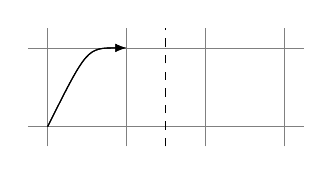
\begin{tikzpicture}
\draw[help lines] (-.25, -.25) grid (3.25, 1.25);
\draw[-latex] (0,0) .. controls (.5,1) .. (1,1);

\draw[dashed] (1.5, -.25) -- (1.5, 1.25);
\pgfexttransformxmirror{1.5}

\draw[-latex] (0,0) .. controls (.5,1) .. (1,1);
\end{tikzpicture}
\end{codeexample}
\end{command}

\switchcolumn% >

\begin{command}{\pgfexttransformxMirror\marg{value}}\cmdcompat\pgftransformxMirror
  Sets up a transformation that mirrors along a vertical line that goes through point $(\text{\meta{value}}, 0)$.

\begin{codeexample}[preamble=\usepgflibrary{ext.transformations.mirror}]
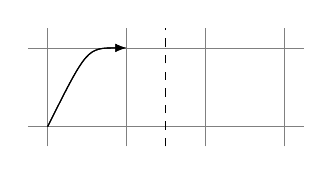
\begin{tikzpicture}
\draw[help lines] (-.25, -.25) grid (3.25, 1.25);
\draw[-latex] (0,0) .. controls (.5,1) .. (1,1);

\draw[dashed] (1.5, -.25) -- (1.5, 1.25);
\pgfexttransformxMirror{1.5}

\draw[-latex] (0,0) .. controls (.5,1) .. (1,1);
\end{tikzpicture}
\end{codeexample}
\end{command}

\switchcolumn*% <

\begin{command}{\pgfexttransformymirror\marg{value}}\cmdcompat\pgftransformymirror
  Sets up a transformation that mirrors along a horizontal line that goes through point $(0, \text{\meta{value})}$.
\end{command}

\begin{command}{\pgfexttransformmirror\marg{point A}\marg{point B}}\cmdcompat\pgftransformmirror
  Sets up a transformation that mirrors along the line that goes through \meta{point A} and \meta{point B}.
 
\begin{codeexample}[preamble=\usepgflibrary{ext.transformations.mirror}]
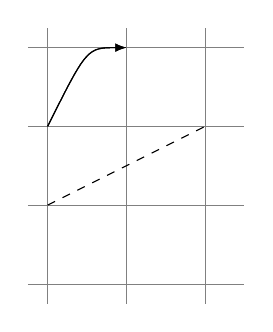
\begin{tikzpicture}
\draw[help lines] (-.25, -2.25) grid (2.5, 1.25);
\draw[-latex] (0,0) .. controls (.5,1) .. (1,1);

\draw[dashed] (0, -1) -- (2, 0);
\pgfexttransformmirror{\pgfpointxy{0}{-1}}
                      {\pgfpointxy{2}{ 0}}

\draw[-latex] (0,0) .. controls (.5,1) .. (1,1);
\end{tikzpicture}
\end{codeexample}
\end{command}

\switchcolumn% >

\begin{command}{\pgfexttransformyMirror\marg{value}}\cmdcompat\pgftransformyMirror
  Sets up a transformation that mirrors along a horizontal line that goes through point $(0, \text{\meta{value})}$.
\end{command}

\begin{command}{\pgfexttransformMirror\marg{point A}\marg{point B}}\cmdcompat\pgftransformMirror
  Sets up a transformation that mirrors along the line that goes through \meta{point A} and \meta{point B}.
 
\begin{codeexample}[preamble=\usepgflibrary{ext.transformations.mirror}]
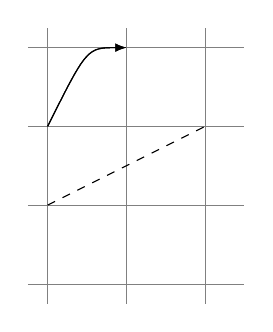
\begin{tikzpicture}
\draw[help lines] (-.25, -2.25) grid (2.5, 1.25);
\draw[-latex] (0,0) .. controls (.5,1) .. (1,1);

\draw[dashed] (0, -1) -- (2, 0);
\pgfexttransformMirror{\pgfpointxy{0}{-1}}
                      {\pgfpointxy{2}{ 0}}

\draw[-latex] (0,0) .. controls (.5,1) .. (1,1);
\end{tikzpicture}
\end{codeexample}
\end{command}

\switchcolumn*% <

\begin{command}{\pgfextqtransformmirror\marg{point A}}\cmdcompat\pgfqtransformmirror
  Sets up a transformation that mirrors along the line that goes through the origin and \meta{point A}.

\begin{codeexample}[preamble=\usepgflibrary{ext.transformations.mirror}]
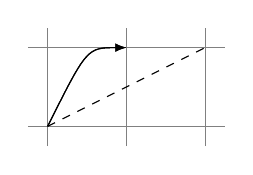
\begin{tikzpicture}
\draw[help lines] (-.25, -.25) grid (2.25, 1.25);
\draw[-latex] (0,0) .. controls (.5,1) .. (1,1);

\draw[dashed] (0, 0) -- (2, 1);
\pgfextqtransformmirror{\pgfpointxy{2}{1}}

\draw[-latex] (0,0) .. controls (.5,1) .. (1,1);
\end{tikzpicture}
\end{codeexample}
\end{command}

\switchcolumn

\begin{command}{\pgfextqtransformMirror\marg{point A}}\cmdcompat\pgfqtransformMirror
  Sets up a transformation that mirrors along the line that goes through the origin and \meta{point A}.

\begin{codeexample}[preamble=\usepgflibrary{ext.transformations.mirror}]
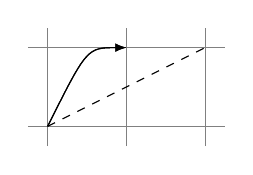
\begin{tikzpicture}
\draw[help lines] (-.25, -.25) grid (2.25, 1.25);
\draw[-latex] (0,0) .. controls (.5,1) .. (1,1);

\draw[dashed] (0, 0) -- (2, 1);
\pgfextqtransformMirror{\pgfpointxy{2}{1}}

\draw[-latex] (0,0) .. controls (.5,1) .. (1,1);
\end{tikzpicture}
\end{codeexample}
\end{command}

\end{paracol}
\endinput

\tikzsetfigurename{PGF.shapes}%
% !TeX spellcheck = en_US
% !TeX root = tikz-ext-manual.tex
% Copyright 2022 by Qrrbrbirlbel
%
% This file may be distributed and/or modified
%
% 1. under the LaTeX Project Public License and/or
% 2. under the GNU Free Documentation License.
%
\section{Shape: Circle Arrow}
\begin{pgflibrary}{ext.shapes.circlearrow}
  A circular shape named |circle arrow| that has an arc as its background path that can have an arrow tip.
  \inspiration{ShapeCircleArrow-Q}{ShapeCircleArrow-A}
\end{pgflibrary}
\begin{shape}{circle arrow}
  This shape is an arrow whose path is an arc -- defined very similar to the |arc|%
  \indexPathOperationO{arc} path operation -- that can possibly be customized with
  arrow tips.
  
  \begin{key}{/pgf/circle arrow start angle=\meta{start angle} (initially \{\})}
  Sets the start angle.
  \end{key}
  \begin{key}{/pgf/circle arrow end angle=\meta{end angle} (initially \{\})}
  Sets the end angle.
  \end{key}
  \begin{key}{/pgf/circle arrow delta angle=\meta{delta angle} (initially \{\})}
  Sets the delta angle.
  \end{key}
  \begin{key}{/pgf/circle arrow arrows=%
    \meta{start arrow tip specification}-\meta{end arrow tip specification} (initially -)}
  The specification will be forwarded to |\pgfsetarrows|\indexCommandO{\pgfsetarrows}.
  \end{key}
  
  A few handful styles are pre-defined.
  \begin{key}{/pgf/circle arrow turn left north}
  Sets |circle arrow start angle = 100|, |circle arrow delta angle = 340|
  and |circle arrow arrows = ->|.
  \end{key}
  \begin{key}{/pgf/circle arrow turn left east}
  As above but |circle arrow start angle = 10|.
  \end{key}
  \begin{key}{/pgf/circle arrow turn left west}
  As above but |circle arrow start angle = 280|.
  \end{key}
  \begin{key}{/pgf/circle arrow turn left south}
  As above but |circle arrow start angle = 190|.
  \end{key}
  \begin{key}{/pgf/circle arrow turn right north}
  Sets |circle arrow start angle = 100|, |circle arrow delta angle = 340|
  and |circle arrow arrows = <-|.
  \end{key}
  \begin{key}{/pgf/circle arrow turn right east}
  As above but |circle arrow start angle = 10|.
  \end{key}
  \begin{key}{/pgf/circle arrow turn right west}
  As above but |circle arrow start angle = 280|.
  \end{key}
  \begin{key}{/pgf/circle arrow turn right south}
  As above but |circle arrow start angle = 190|.
  \end{key}

{\catcode`\|=12
\begin{codeexample}[preamble=\usetikzlibrary{ext.shapes.circlearrow,matrix}]
\begin{tikzpicture}
\matrix[matrix of nodes, draw=none, row sep=1em, column sep=1em,
  every node/.style={draw=gray, shape=circle arrow, ultra thick, inner sep=1em}
] (m) {
  |[circle arrow turn left north]|  & |[circle arrow turn left east]|   \\
  |[circle arrow turn left west]|   & |[circle arrow turn left south]|  \\
  |[circle arrow turn right north]| & |[circle arrow turn right east]|  \\
  |[circle arrow turn right west]|  & |[circle arrow turn right south]| \\
};
\end{tikzpicture}
\end{codeexample}
}
\begin{codeexample}[preamble=\usetikzlibrary{ext.shapes.circlearrow},width=16cm]
\begin{tikzpicture}\Huge
\node[name=s, shape=circle arrow,
  circle arrow turn left west, shape example]
  {Circle Arrow\vrule width 1pt height 2cm};
\foreach \anchor/\placement in
  {north west/above left, north/above,
   north east/above right,
   west/left, center/above, east/right,
   mid west/right, mid/above, mid east/left,
   base west/left, base/below, base east/right,
   south west/below left, south/below,
   south east/below right,
   text/left, 10/right, 130/above}
   \draw[shift=(s.\anchor)] plot[mark=x] coordinates{(0,0)}
     node[\placement] {\scriptsize\texttt{(s.\anchor)}};
\end{tikzpicture}
\end{codeexample}
\end{shape}
\endinput
% !TeX spellcheck = en_US
% !TeX root = tikz-ext-manual.tex
% Copyright 2022 by Qrrbrbirlbel
%
% This file may be distributed and/or modified
%
% 1. under the LaTeX Project Public License and/or
% 2. under the GNU Free Documentation License.
%
\section{Shape: Circle Cross Split}
\begin{pgflibrary}{ext.shapes.circlecrosssplit}
  A circular shape with four parts that can be individually filled.
\end{pgflibrary}
\begin{key}{/pgf/circle cross split part fill=\marg{list} (initially |none|)}
Sets the custom fill color for each node part shape.
The items in \meta{list} should be separated by commas
(so if there is more than one item in \meta{list}, it must be surrounded by braces).
If \meta{list} has less entries than node parts,
then the remaining node parts use the color from the last entry in the list.
This key will automatically set |/pgf/circle cross split uses custom fill|.
\end{key}
\begin{key}{/pgf/circle cross split uses custom fill=\opt{\meta{boolean}} (default |true|)}
This enables the use of a custom fill for each of the node parts
(including the area covered by the |inner sep|).
The background path for the shape should not be filled (e.\,g., in \tikzname,
the |fill| option for the node must be implicitly or explicitly set to |none|).
Internally, this key sets the TeX-if |\ifpgfcirclecrosssplitcustomfill| appropriately. 
\end{key}
\begin{codeexample}[preamble=\usepgflibrary{ext.shapes.circlecrosssplit}]
\begin{tikzpicture}\Huge
\node[name=s, shape=circle cross split, shape example, inner xsep=1.5cm,
  circle cross split part fill={green,blue,red,yellow!90!black}]
 {\nodepart{text}text\nodepart{two}two
         \nodepart{three}three\nodepart{four}four};
\foreach \anchor/\placement in
    {north west/above left, north/above,      north east/above right,
           west/left,      center/above,            east/right,
       mid west/right,        mid/left,         mid east/left,
      base west/left,        base/left,        base east/right,
lower base west/left,  lower base/below, lower base east/right,
 lower mid west/left,  lower mid/above,   lower mid east/right,
     south west/below left, south/below,      south east/below right,
   text/below, 10/right, 130/above, two/left, three/left, four/left}
   \draw[shift=(s.\anchor)] plot[mark=x] coordinates{(0,0)}
     node[\placement] {\scriptsize\texttt{(s.\anchor)}};
\end{tikzpicture}
\end{codeexample}

% !TeX spellcheck = en_US
% !TeX root = tikz-ext-manual.tex
% Copyright 2022 by Qrrbrbirlbel
%
% This file may be distributed and/or modified
%
% 1. under the LaTeX Project Public License and/or
% 2. under the GNU Free Documentation License.
%
\section{Shape: Heatmark}
\begin{pgflibrary}{ext.shapes.heatmark}
  A circular shape that has customizable rings around it.
  \inspiration{ShapeHeat-Q}{ShapeHeat-A}
\end{pgflibrary}

\begin{ext_shape}{heatmark}
  \begin{key}{/\pgfext/heatmark arcs=\meta{arcs num} (initially 3)}\keycompat{pgf}
  Sets the number of arc around the circle to \meta{arcs num}.
  \end{key}
  \begin{key}{/\pgfext/heatmark arc width=\meta{arc width} (initially 4pt)}\keycompat{pgf}
  Sets the width of the rings around the circle to \meta{arc width}.
  \end{key}
  \begin{key}{/\pgfext/heatmark arc sep=\meta{sep length} (initially 1pt)}\keycompat{pgf}
  Sets the whitespace between the rings to \meta{sep length}.
  \end{key}
  \begin{key}{/\pgfext/heatmark arc rings=\meta{rings num} (initially 3)}\keycompat{pgf}
  Sets the number of rings around the circle to \meta{rings num}
  \end{key}
  \begin{key}{/\pgfext/heatmark arc sep angle=\meta{sep angle} (initially 20)}\keycompat{pgf}
  Sets the whitespace angle between the arcs in one ring to \meta{sep angle}.
  \end{key}
  \begin{key}{/\pgfext/heatmark inner opacity=\meta{inner opacity} (initially 0.8)}\keycompat{pgf}
  Sets the opacity of the inner ring to \meta{inner opacity}.
  \end{key}
  \begin{key}{/\pgfext/heatmark outer opacity=\meta{low opacity} (initially 0.2)}\keycompat{pgf}
  Sets the opacity of the outer ring to \meta{outer opacity}.
  
  The opacity of the rings between the outer and the inner ring will be interpolated by these two opacities.
  \end{key}

This shape takes the value of |/pgf/shape border rotate|%
\indexKeyO[/pgf/]{shape border rotate} into consideration.

For every ring and for every arc the following styke keys are tried.
\begin{stylekey}{/\pgfext/heatmark ring \meta{ring number}}
\end{stylekey}
\begin{stylekey}{/\pgfext/heatmark arc \meta{arc number}}
\end{stylekey}
\begin{stylekey}{/\pgfext/heatmark ring \meta{ring number} arc \meta{arc number}}
\end{stylekey}

The \pgfname shape is setup in a way that even \tikzname\space
styles can be used with a little bit work:
\begin{codeexample}[preamble=\usetikzlibrary{ext.shapes.heatmark}]
\tikz[
  shape border rotate=90,
  /pgf/ext/heatmark ring 1/.append style={/tikz/fill=green},
  /pgf/ext/heatmark arc 1/.append style={/tikz/fill=blue},
  /pgf/ext/heatmark ring 2 arc 2/.append style={/tikz/fill=yellow!70!black}
] \node[ext_heatmark, fill=red] (n) {100};
\end{codeexample}

It is best to use this shape with no actual border (|draw = none|) and the |outer sep| set to zero.
\begin{codeexample}[preamble=\usetikzlibrary{ext.shapes.heatmark},width=16cm]
\begin{tikzpicture}\Huge
\node[name=s, shape=ext_heatmark, shape example,
  fill=blue!25, draw=none, outer sep=0pt]
  {Heatmark\vrule width 1pt height 2cm};
\foreach \anchor/\placement in
  {north west/above left, north/above,
                          north east/above right,
         west/left, center/above,      east/right,
     mid west/right,   mid/above,  mid east/left,
    base west/left,   base/below, base east/right,
   south west/below left, south/below,
                          south east/below right,
   text/left, 10/right, 130/above}
   \draw[shift=(s.\anchor)] plot[mark=x] coordinates{(0,0)}
     node[\placement] {\scriptsize\texttt{(s.\anchor)}};
\end{tikzpicture}
\end{codeexample}
\end{ext_shape}
\endinput
% !TeX spellcheck = en_US
% !TeX root = tikz-ext-manual.tex
% Copyright 2022 by Qrrbrbirlbel
%
% This file may be distributed and/or modified
%
% 1. under the LaTeX Project Public License and/or
% 2. under the GNU Free Documentation License.
%

\section{Shape: Rectangle with Rounded Corners}
\begin{pgflibrary}{ext.shapes.rectangleroundedcorners}
  A rectangle with rounded corners.
\end{pgflibrary}

\begin{key}{/pgf/rectangle with rounded corners north west radius=\meta{dimen} (initially .5\string\pgflinewidth)}
  Sets the north west radius to \meta{dimen}.
\end{key}
\begin{key}{/pgf/rectangle with rounded corners north east radius=\meta{dimen} (initially .5\string\pgflinewidth)}
  Sets the north east radius to \meta{dimen}.
\end{key}
\begin{key}{/pgf/rectangle with rounded corners south west radius=\meta{dimen} (initially .5\string\pgflinewidth)}
  Sets the south west radius to \meta{dimen}.
\end{key}
\begin{key}{/pgf/rectangle with rounded corners south east radius=\meta{dimen} (initially .5\string\pgflinewidth)}
  Sets the south east radius to \meta{dimen}.
\end{key}
\begin{key}{/pgf/rectangle with rounded corners radius=\meta{dimen}}
  Sets all radii to \meta{dimen}.
\end{key}

\begin{codeexample}[preamble=\usepgflibrary{ext.shapes.rectangleroundedcorners}]
\tikzexternaldisable
\begin{tikzpicture}\Huge
\node[name=s, shape=rectangle with rounded corners, shape example,
  rectangle with rounded corners north west radius=10pt,
  rectangle with rounded corners north east radius=20pt,
  rectangle with rounded corners south west radius=30pt,
  rectangle with rounded corners south east radius=40pt] {Rectangle with rounded corners\vrule width 1pt height 2cm};
\foreach \anchor/\placement in
  {north west/above left, north/above, north east/above right,
         west/left,      center/above,       east/right,
     mid west/right,        mid/above,   mid east/left,
    base west/left,        base/below,  base east/right,
   south west/below left, south/below, south east/below right,
   text/left,% 10/right, 130/above,
   north west center/below right,      north east center/below left,
   south west center/above right,      south east center/above left}
   \draw[shift=(s.\anchor)] plot[mark=x] coordinates{(0,0)}
     node[\placement] {\scriptsize\texttt{(s.\anchor)}};
\end{tikzpicture}
\end{codeexample}
% !TeX spellcheck = en_US
% !TeX root = tikz-ext-manual.tex
% Copyright 2022 by Qrrbrbirlbel
%
% This file may be distributed and/or modified
%
% 1. under the LaTeX Project Public License and/or
% 2. under the GNU Free Documentation License.
%

\section{Shape: Superellipse}
\begin{pgflibrary}{ext.shapes.superellipse}
  Shape in the form of a ``superellipse''.
\end{pgflibrary}

\begin{shape}{superellipse}
This shape is defined by formula
\begin{equation*}
  \biggl|\frac x{r_x}\biggr|^m + \biggl|\frac y{r_y}\biggr|^n = 1
\end{equation*}
and will be plotted by
\begin{align*}
  x(t) &= |\cos t|^{\frac 2m} \cdot r_x \sgn(\cos t) \\
  y(t) &= |\sin t|^{\frac 2n} \cdot r_y \sgn(\sin t) \\
\end{align*}
where $r_x$ is half the node's width and $r_y$ is half the node's height.

\begin{key}{/pgf/superellipse x exponent=\meta{x exponent}(initially 2.5)}
This sets $m$.
\end{key}
\begin{key}{/pgf/superellipse y exponent=\meta{y exponent}(initially 2.5)}
This sets $n$.
\end{key}
\begin{key}{/pgf/superellipse step=\meta{step}(initially 5)}
This specifies the step of the underlying plot handler.
The smaller \meta{step} is, the slower computation will be.

Sensible values for \meta{step} are integer dividers of 90, i.\,e.
2, 3, 5, 6, 9, 10, 15, 18, 30 and 45.
\end{key}
\begin{key}{/pgf/superellipse exponent=\meta{exponent}}
  Sets both |superellipse x exponent| and |superellipse y exponent| to \meta{exponent}.
\end{key}

\paragraph{Notes on Implementation}
For implementing this shape, additional mathematical functions were declared.
\begin{math-function}{superellipsex(\mvar{t}, \mvar{2/m}, \mvar{$r_x$})}
\mathcommand
Returns the $x$ value on a point of the superellipse with its center on the origin following
\begin{equation*}
   x = r_x\cos^{2/m} t
\end{equation*}
for values of $0 \leq t \leq 90$.
\end{math-function}
\begin{math-function}{superellipsey(\mvar{t}, \mvar{2/n}, \mvar{$r_y$})}
\mathcommand
Returns the $y$ value on a point of the superellipse with its center on the origin following
\begin{equation*}
   y = r_y\cos^{2/n} t
\end{equation*}
for values of $0 \leq t \leq 90$.
\end{math-function}

Both \pgfname math functions can be used at once with the following macro.
\begin{command}{\pgfmathsuperellipseXY\marg{t}\marg{2/m}\marg{2/n}\marg{a}\marg{b}}
Returns the $x$ value (in |\pgfmathresultX|) and the $y$ value (in |\pgfmathresultY|) of the superellipse with its center on the origin following
\begin{align*}
   x & = a\cos^{2/m} t \\
   y & = b\cos^{2/n} t
\end{align*}
for values of $0 \leq t \leq 90$.

Note: all arguments must be a valid number since they will not be parsed by \pgfname math.
\end{command}

And additional internal macro was defined following the original naming scheme.
\def\temp{\begin{command}}%
\expandafter\temp\expandafter{\csname pgfutil@prefix@macrotomacro\endcsname\marg{macro 1}\marg{macro 2}}
Adds the once-expansion of \meta{macro 2} in front of \meta{macro 1}.
\end{command}

\begin{codeexample}[preamble=\usetikzlibrary{ext.shapes.superellipse}]
\begin{tikzpicture}[superellipse step=1]\Huge
\node[name=s,shape=superellipse,shape example] {Superellipse\vrule width 1pt height 2cm};
\foreach \anchor/\placement in
  {north west/above left, north/above, north east/above right,
   west/left, center/above, east/right,
   mid west/right, mid/above, mid east/left,
   base west/left, base/below, base east/right,
   south west/below left, south/below, south east/below right,
   text/left, 10/right, 130/above}
   \draw[shift=(s.\anchor)] plot[mark=x] coordinates{(0,0)}
     node[\placement] {\scriptsize\texttt{(s.\anchor)}};
\end{tikzpicture}
\end{codeexample}
%
\begin{codeexample}[width=8cm,preamble=\usetikzlibrary{ext.shapes.superellipse}]
\begin{tikzpicture}[minimum width=1cm, minimum height=3cm]
\foreach \xe/\ye[count=\i] in {.5/.5, 1/1, 2/2, 3/3, .5/5}
  \node[draw, superellipse, superellipse x exponent=\xe, superellipse y exponent=\ye] at (1.5*\i,0) {};
\end{tikzpicture}
\end{codeexample}
\end{shape}
\endinput
% !TeX spellcheck = en_US
% !TeX root = tikz-ext-manual.tex
% Copyright 2022 by Qrrbrbirlbel
%
% This file may be distributed and/or modified
%
% 1. under the LaTeX Project Public License and/or
% 2. under the GNU Free Documentation License.
%

\section{Shape: Uncentered Rectangle}
\begin{purepgflibrary}{ext.shapes.uncenteredrectangle}
  A rectangle that has a variable horizontal center with three node parts.
  \inspiration{UncRectCD-Q,UncRectForest-Q}{UncRectCD-A,UncRectForest-A}
\end{purepgflibrary}
\begin{shape}{uncentered rectangle}

For some alignment problems, this shape could be useful.

It has three node parts: the standard |text| part,
the |left| part that is to the left of |text|
and the |right| part that is to the right of |text|.

When edges are to be connected with this shape, the
following key changes to which inner center this shape will
calculate the appropriate point on the border.
\begin{key}{/pgf/uncentered rectangle center=\meta{left}\textrm{ or }\meta{text}\textrm{ or }\meta{right}\textrm{ or }\meta{real} (initially text)}
  Sets the center that is to be used for connecting edges.
  
  This will also move the anchors |north|, |mid|, |base| and |south| along.
  In the picture below, this are marked red.
\end{key}

\begin{key}{/pgf/uncentered rectangle use saved center=\meta{true}\textrm{ or }\meta{false} (default true)}
When this is set to true, the border anchors will use the horizontal center that was used when
the node was created.
\end{key}

For support of the \referenceLibraryandIndexO{cd} library of the |tikz-cd| package,
this shape also supports a dynamic $y$ value for its anchors |center|, |west| and |east|.
\begin{key}{/pgf/uncentered rectangle center yshift=\meta{dimension} (initially \{\})}
  This determines the distance between the baseline and the |center| anchors.
  
  If \meta{dimension} is empty, the real vertical center will be used.
  
  For use with |cd|, set this to |axis_height|.
\end{key}
%\pagebreak
\begin{codeexample}[preamble=\usepgflibrary{ext.shapes.uncenteredrectangle}]
\begin{tikzpicture}[style north/.style=red, style south/.style=red, style center/.style=red, style base/.style=red, style mid/.style=red]
\Huge
\node[shape example, name=n, uncentered rectangle]
  {centered \nodepart{left} Un \nodepart{right} \space Rectangle\vrule width 1pt height 2cm}
  foreach \anchor/\pos in {
   north west/above left, north/below, north east/above right, real north/above,  left north/above, right north/above, text north/above,
         west/left,      center/above,       east/right,       real center/above, left center/above,right center/above,text center/below,
     mid west/left,         mid/left,    mid east/right,       real mid/above,    left mid/above,   right mid/above,   text mid/above,
    base west/left,        base/right,  base east/right,       real base/below,   left base/below,  right base/below,  text base/below,
   south west/below left, south/above, south east/below right, real south/below,  left south/below, right south/below, text south/below,
                             10/right,        130/below,                          left/left,        right/right,       text/right}{
    plot[mark=x, only marks] coordinates {(n.\anchor)}
    node[inner sep=.1em, style \anchor/.try, style/.expand once=\pos] {\tiny\ttfamily\anchor}};
\end{tikzpicture}
\end{codeexample}
\end{shape}

\begin{tikzlibrary}{ext.shapes.uncenteredrectangle}
This library extends the \referenceLibraryandIndexO{cd} library (from the |tikz-cd| package)
so that it can be used with the |uncentered rectangle| shape.

\inspirationQ{UncRectCD2-Q}
\end{tikzlibrary}

This library provides only one key.
\begin{stylekey}{/tikz-ext/tikz-cd fix}
This key installs various \enquote{fixes} to the \referenceKeyandIndexO[/tikz/commutative diagrams/]{every diagram} style:

\begin{itemize}
\item Firstly, is defines a \referenceKeyandIndexO{matrix of math nodes} key (only for the \referenceEnvironmentandIndexO{tikzcd} environment)
      which allows to toggle the \referenceKeyandIndexO[/tikz/commutative diagrams/]{math mode} for each node.%
      \footnote{Due to a bug with \referenceKeyandIndexO{execute at end node}, the \enquote{automatic} math mode in matrices can't be used
        with multipart nodes.}
\item The helpful macro |\uncrec| will be installed.
\begin{command}{\uncrec\marg{left}\marg{center}\marg{right}}
  When used as the content of |uncentered rectangle|,
  the node parts will be setup so that \meta{left} is in the left part of the node part etc.
\end{command}
\item Since math mode will be disabled with the |uncentered rectangle|, it is automatically enabled for each node part with |\uncrec| but it can be disabled with the following key.
\begin{key}{/tikz/uncrec math mode=\meta{true}\textrm{ or }\meta{false} (default true)}
When enabled the contents of |\uncrec| will be set in math mode.
\end{key}
\item For easy access to the |uncentered rectangle| shape, the following keys are available inside a Commutative Diagram.
\begin{stylekey}{/tikz/uncrec=\meta{left}\textrm{ or }\meta{text}\textrm{ or }\meta{right}\textrm{ or }\meta{real} (initially text)}
This key sets the shape to |uncentered rectangle| and \referenceKeyandIndex[/pgf/]{uncentered rectangle center} to its argument.
\end{stylekey}
\begin{stylekey}{/tikz/commutative diagrams/install uncentered rectangle in columns=\meta{column}}
All nodes in column \meta{column} will be set to the |uncentered rectangle| shape.
\end{stylekey}
\end{itemize}
\end{stylekey}

\begingroup
\tikzexternaldisable
%\catcode`\|=12
\begin{codeexample}[leave comments, width=8cm, preamble=\usetikzlibrary{cd, ext.shapes.uncenteredrectangle}]
\tikzcdset{/tikz-ext/tikz-cd fix}
\newcommand*\C[1]{C_{\%_{#1}}}
\begin{tikzcd}[
  sep=tiny,
  arrows={-, gray},
  cells={font=\strut, inner xsep=.2ex, inner ysep=.1ex},
  install uncentered rectangle in column=3
]
\C{1} \drar &         & \uncrec{}{m_{r_1}}{{} = \C{2}-C_\%} \dlar\\
            & C_\% \\
\C{2} \urar &         & \uncrec{}{m_{r_2}}{{} = \C{1}-C_\%} \ular
\end{tikzcd}
\end{codeexample}
\begin{codeexample}[leave comments, width=8cm, preamble=\usetikzlibrary{cd, ext.shapes.uncenteredrectangle}]
\tikzset{/tikz-ext/tikz-cd fix}
\begin{tikzcd}[install uncentered rectangle in column/.list={1,2}]
  \uncrec{S \supset {}}{U_\tau}{}                                      \arrow[r, "\varphi_0"]
                                                                       \arrow[d, "\tau", "\sim"']
& \uncrec{}{U_\pi}{{} \subset T}                                       \arrow[d, "\pi",  "\sim"']
\\
  \uncrec{\operatorname{Bl}_{(0,0)}(\mathbb{A}^2) \supset{}}{V_\tau}{} \arrow[r, "\epsilon"]
& \uncrec{}{V_\pi}{{} \subset \mathbb{A}^2}
\end{tikzcd}
\end{codeexample}
\endgroup
\endinput

\part{Utilities}

\label{part:misc}
\vfill\tikzsetnextfilename{main-misc}
\begin{codeexample}[width=6cm, preamble=\usetikzlibrary{ext.misc}]
\begin{tikzpicture}[
  declare function={bigR(\n)=smallR+.05*\n;},
  ext/declare constant={smallR=1; segments=20;},
  ext/full arc=segments]
\foreach \iN[evaluate={\endRadius=bigR(\iN+1);}, ext/use int=0 to segments-1]
  \filldraw[fill=gray!50] (\iN R:\endRadius)
    arc [radius=\endRadius, start angle=\iN R, delta angle=+1R] -- (\iN R+1R:smallR)
    arc [radius=smallR,       end angle=\iN R, delta angle=-1R] -- cycle;

\node                                              {$\phi^2$};
\node at (north west:{sqrt 2 * bigR(segments/2)})  {$\{\Omega\}_{i=1}^n$};
\node[rotate=-.5R, right] at (-.5R: bigR segments) {$\partial \varphi$};

\tikzset{yshift=-5cm, ext/declare constant={segments=25;}, ext/full arc=segments}
\filldraw[fill=gray!50] (right:smallR)
  \foreach \iN[evaluate={\endRadius=bigR(\iN+1);}, ext/use int=0 to segments-1] {
    -- (\iN R:\endRadius) arc[radius=\endRadius, start angle=\iN R, delta angle=1R]}
    -- (right:smallR)     arc[radius=smallR,     start angle=0,     delta angle=-360];

\node                                              {$\phi^2$};
\node at (north west:{sqrt 2 * bigR(segments/2)})  {$\{\Omega\}_{i=1}^n$};
\node[rotate=-.5R, right] at (-.5R: bigR segments) {$\partial \varphi$};
\end{tikzpicture}
\end{codeexample}
\vfill

\tikzsetfigurename{misc.calendar}% !TeX spellcheck = en_US
% !TeX root = tikz-ext-manual.tex
% Copyright 2022 by Qrrbrbirlbel
%
% This file may be distributed and/or modified
%
% 1. under the LaTeX Project Public License and/or
% 2. under the GNU Free Documentation License.
%

\section{Calendar: Weeknumbers and more conditionals}
\begin{package}{calendar-ext}
  This package adds week numbers and more conditionals to the \pgfname\space package |pgfcalendar|.
  (Despite the code example above, this package is not set up to work with Con\TeX t.)
\end{package}

%This package extends the |pgfcalendar| package.

\begin{multicols}{2}

\subsection{Extensions}

The following tests are added.
\begin{itemize}
\itemcalendaroption{Jan} This test is passed by all dates that are in the month of January.
\itemcalendaroption{Feb} as above.
\itemcalendaroption{Mar} as above.
\itemcalendaroption{Apr} as above.
\itemcalendaroption{May} as above.
\itemcalendaroption{Jun} as above.
\itemcalendaroption{Jul} as above.
\itemcalendaroption{Aug} as above.
\itemcalendaroption{Sep} as above.
\itemcalendaroption{Oct} as above.
\itemcalendaroption{Nov} as above.
\itemcalendaroption{Dec} as above.
\itemcalendaroption{leap year}\opt{|=|\meta{year}}
    This test checks whether the given year is a leap year. If
    \meta{year} is omitted, it checks the year of the current date.
\itemcalendaroption{and}|=|\marg{tests}
    This test passes when all \meta{tests} pass.
\itemcalendaroption{not}|=|\marg{tests}
    This test passes when \meta{tests} do not pass.
\itemcalendaroption{yesterday}|=|\marg{tests}
    This test passes when the previous day passes \meta{tests}.
\itemcalendaroption{week}|=|\meta{num}
    This test passes when the current week of the year equals \marg{num}.
\end{itemize}

The shorthands for |d-| and |m-| are slightly changed so that they are
expandable. This makes it possible to use these shorthands inside of \pgfname math.
The shorthands for the week (see section~\ref{calendar:weeknumbering})
are added. These are
\begin{itemize}
\item |n-| (shortest numerical representation),
\item |n=| (shortest but added horizontal space) and
\item |n0| (leading zero when below 10).
\end{itemize}

\subsection{Week numbering (ISO~8601)}
\label{calendar:weeknumbering}
\begin{command}{\pgfcalendarjulianyeartoweek\marg{Julian day}\marg{year}\marg{week counter}}
  This command calculates the week for the \meta{Julian day} of \meta{year}.
  The \meta{week counter} must be a \TeX\space counter.

  The calculation follows the rule of ISO~8601 where the first week has that
  year's first Thursday in it.
\end{command}

Inside of |\pgfcalendar|\indexCommandO\pgfcalendar the command |\pgfcalendarcurrentweek| will be available.
\begin{command}{\pgfcalendarcurrentweek}
  This command returns the current week number (always two digits -- use shorthand |n.|
  to strip the leading zero).
\end{command}

Inside of |\ifdate|\indexCommandO\ifdate the command |\pgfcalendarifdateweek| will be available.
\begin{command}{\pgfcalendarifdateweek}
  This command returns the week number (always two digits).
\end{command}
\end{multicols}
\tikzsetfigurename{misc.pgffor}% !TeX spellcheck = en_US
% !TeX root = tikz-ext-manual.tex
% Copyright 2022 by Qrrbrbirlbel
%
% This file may be distributed and/or modified
%
% 1. under the LaTeX Project Public License and/or
% 2. under the GNU Free Documentation License.
%
\section{Repeating Things and Other Things}
\label{pkg:pgffor-ext}
\begin{texpackage}{pgffor-ext}
  This package adds small niceties to the \referencePackageandIndexO{pgffor} package.
  Most of these additions are also available
  with the \referenceLibraryandIndex{ext.misc} library.

  \textbf{Warning:} Consider this package experimental.
  At the very least, it will break the |...| notation and possibly gobbles spaces after the body.
  
  \inspiration{ForeachUse-Q, ForeachNoSep-Q, ForeachXparse-Q}{ForeachUse-A, ForeachNoSep-A, ForeachXparse-A}
\end{texpackage}

Instead of |\foreach \var in {start, start + delta, ..., end}| one can use
|\foreach \var[use int=start to end step delta]|.

\begin{key}{/pgf/foreach/use int=\meta{start}|to|\meta{end}\opt{|step|\meta{delta}}}
The values \meta{start}, \meta{end} and \meta{delta} are evaluates by \pgfname math at initialization.
The part |step |\meta{delta} is optional (\meta{delta} = 1).
\end{key}

\begin{key}{/pgf/foreach/use float=\meta{start}|to|\meta{end}\opt{|step|\meta{delta}}}
Same as above, however the results are not truncated.
\end{key}

\begin{key}{/pgf/foreach/no separator}
This key disables any separator between elements of the list.
Every token is its own element. This also means that Unicode characters
need to be grouped between |{| and |}| if Lua\TeX\space isn't used.
Spaces will be ignored.

\begin{codeexample}[preamble=\usetikzlibrary{ext.misc}]
\newcommand*{\board}[3][]{%
  \begin{tikzpicture}[#1]
    \foreach[
      count=\i from 0,
      no separator,
      evaluate=\i as \colX using {mod(\i,#2)},
      evaluate=\i as \rowY using {int(\i/#2)}
    ] \elem in {#3} {
        \draw[black, board/\elem/.try, ext/rectangle timer/.try=line]
          (\colX,\rowY) rectangle node {\elem} ++(1, 1);}
  \end{tikzpicture}}
\board[
  board/W/.style={fill=red},
  board/X/.style={fill=blue!50},
  board/B/.style={fill=green},
  board/-/.style={fill=gray},
]{3}{WXX---BXX}
\end{codeexample}
\end{key}

\begin{key}{/pgf/foreach/normal list}
This key simply disables all other special parsers and returns to the original list parser.
\end{key}

The following keys only work with \LaTeX\ and cannot be used when only the \referenceLibraryandIndex{ext.misc}
library or the plain\TeX\space |pgffor-ext.tex| are loaded.
For this, you will need to use |\usepackage{pgffor-ext}|.
\begin{key}{/pgf/foreach/xparser=\marg{argument specification}\marg{foreach value}}
This key can be used to specify a \referencePackageandIndeXExt{xparse}
specification for each element in the list.

For this to work somewhat seamless, the following needs to observed:
\begin{itemize}
  \item Every \marg{argument specification} get appended |u,|.
        This means there's always one additional mandatory argument at the end of every element.
  \item The \marg{foreach value} needs to correspond to the
        \referenceKeyandIndexO[/pgf/foreach/]{var}
        value.
\end{itemize}
\end{key}

\begin{key}{/pgf/foreach/xparser Om}
Sets up a list whose elements may contain an optional argument inside |[]| which correspond to
two |\foreach| variables, say |\Options/\Text|.
\end{key}

\begin{handler}{{.list xparse}|=|\marg{argument specification}\marg{comma-separated list of values}}
  This handler causes the key to be used repeatedly, namely
  once for every element of the list of values.
  The \meta{comma-separated list of values} is processed using |\foreach|
  and the given |xparse| \meta{argument specification} with the aforementioned |xparser| key.
\end{handler}

\tikzsetfigurename{misc.misc}% !TeX spellcheck = en_US
% !TeX root = tikz-ext-manual.tex
% Copyright 2022 by Qrrbrbirlbel
%
% This file may be distributed and/or modified
%
% 1. under the LaTeX Project Public License and/or
% 2. under the GNU Free Documentation License.
%

\begin{tikzlibrary}{misc}
  This library adds miscelleaneos utilities to PGFmath, PGF or \tikzname.
\end{tikzlibrary}

\section{PGFmath}

\subsection{Postfix operator \texttt{R}}

Similar to |\segments[<num>]| in PSTricks, the postfix operator |R| allows the user
to use an arbitrary number of segments of a circle to be used instead of an angle.

\begin{key}{/tikz/full arc=\meta{num} (default |{}|)}
  The number \meta{num} of segments will be set up.
  Using |full arc| with an empty value disables the segmentation and |1R| equals $1^\circ$.
  
  The given value \meta{num} is evaluated when the key is used and doesn't change when
  \meta{num} contains variables that change.
\end{key}
The |R| operator can then be used.
\begin{math-operator}{R}{postfix}{fullarc}
  Multiplies \mvar{x} with $\frac{360}{\meta{num}}$.
\end{math-operator}

\subsection{Functions}

\begin{math-function}{strrepeat("\mvar{Text}", \mvar{x})}
\mathcommand
  Returns a string with \mvar{Text} repeated \mvar{x} times.

\begin{codeexample}[]
\pgfmathparse{strrepeat("foo", 5)} \pgfmathresult
\end{codeexample}
\end{math-function}

\begin{math-function}{isInString("\mvar{String}", "\mvar{Text}")}
\mathcommand
  Returns |1| (true) if \mvar{Text} contains \mvar{String},
  otherwise |0| (false).

\begin{codeexample}[]
\pgfmathparse{isInString("foo", "bar")} \pgfmathresult
\ and\ 
\pgfmathparse{isInString("foo", "foobar")} \pgfmathresult
\end{codeexample}
\end{math-function}

\begin{math-function}{strcat("\mvar{Text A}", "\mvar{Text B}", …)}
\mathcommand
  Returns the concatenation of all given parameters.

\begin{codeexample}[]
\pgfmathparse{strcat("blue!", int(7*3), "!green")} \pgfmathresult
\end{codeexample}
\end{math-function}


\begin{math-function}{isEmpty("\mvar{Text}")}
\mathcommand
  Returns |1| (true) if \mvar{Text} is empty, otherwise |0| (false).
  %
\begin{codeexample}[]
\pgfmathparse{isEmpty("foo")} \pgfmathresult\ and\ 
\pgfmathparse{isEmpty("")}    \pgfmathresult\ and\ 
\def\emptyText{}
\pgfmathparse{isEmpty("\emptyText")} \pgfmathresult
\end{codeexample}
\end{math-function}

\begin{math-function}{atanXY(\mvar{x},\mvar{y})}
\mathcommand
  Arctangent of $\mvar y\div \mvar x$ in degrees. This also takes into account the quadrant.
  This is just a argument-swapped version of |atan2| which makes it easier to use
  the |\p| commands of the |calc| library.
  \index{atan2@\protect\texttt{atan2} math function}%
  \index{Math functions!atan2@\protect\texttt{atan2}}%
  %
\begin{codeexample}[]
\pgfmathparse{atanXY(3,4)} \pgfmathresult
\end{codeexample}
\end{math-function}
\begin{math-function}{atanYX(\mvar{y},\mvar{x})}
\mathcommand
   Arctangent of $y\div x$ in degrees. This also takes into account the quadrant.
\begin{codeexample}[]
\pgfmathparse{atanYX(4,3)} \pgfmathresult
\end{codeexample}
\end{math-function}

\subsection{Functions: using coordinates}
The following functions can only be used with PGF and/or \tikzname.
Since the arguments are usually plain text (and not numbers) one has to wrap
them in |"|.
\begin{math-function}{anglebetween("\mvar{p1}", "\mvar{p2}")}\mathcommand
  Return the angle between the centers of the nodes \mvar{p1} and \mvar{p2}.
\end{math-function}
\begin{math-function}{qanglebetween("\mvar{p}")}\mathcommand
  Return the angle between the origin and the center of the node \mvar{p}.
\end{math-function}
\begin{math-function}{distancebetween("\mvar{p1}", "\mvar{p2}")}\mathcommand
  Return the distance (in pt) between the centers of the nodes \mvar{p1} and \mvar{p2}.
\end{math-function}
\begin{math-function}{qdistancebetween("\mvar{p}")}\mathcommand
  Return the distance (in pt) between the origin and the center of the node \mvar{p}.
\end{math-function}
\begin{codeexample}[width=6cm,preamble=\usetikzlibrary{calc,misc,through}]
\begin{tikzpicture}
\path (0,0) coordinate (A) + (0:4) coordinate (B) +(75:4) coordinate (C);
\draw (A) -- (B) -- (C) -- cycle;
\foreach \cnt in {1,...,4}{
  \pgfmathsetmacro\triA{distancebetween("B","C")}
  \pgfmathsetmacro\triB{distancebetween("C","A")}
  \pgfmathsetmacro\triC{distancebetween("A","B")}
  \path (barycentric cs:A=\triA,B=\triB,C=\triC) coordinate (M)
       node [draw, circle through=($(A)!(M)!(C)$)] (M) {};
  \draw ($(C)-(A)$) coordinate (vecB)
      (M.75-90) coordinate (@)
      (intersection of @--[shift=(vecB)]@ and B--C) coordinate (C) -- 
      (intersection of @--[shift=(vecB)]@ and B--A) coordinate (A);}
\end{tikzpicture}
\end{codeexample}
\section{PGFkeys}

\subsection{Conditionals}

\begin{key}{/utils/if=\meta{cond}\meta{true}\opt{\meta{false}}}
  This key checks the conditional \meta{cond} and applies the styles \meta{true}
  if \meta{cond} is true, otherwise \meta{false}.
  \meta{cond} can be anything that PGFmath understands.
  
  As a side effect on how PGFkeys parses argument, the \meta{false} argument is
  actually optional.
\end{key}

The following keys use \TeX' macros |\if|, |\ifx|, |\ifnum| and |\ifdim| for faster
executions.

\begin{key}{/utils/TeX/if=\meta{token A}\meta{token B}\meta{true}\opt{\meta{false}}}
  This key checks via |\if| if \meta{token A} matches \meta{token B}
  and applies the styles \meta{true} if it does, otherwise \meta{false}.
  
  As a side effect on how PGFkeys parses argument, the \meta{false} argument is
  actually optional.
\end{key}

\begin{key}{/utils/TeX/ifx=\meta{token A}\meta{token B}\meta{true}\opt{\meta{false}}}
  As above.
\end{key}

\begin{key}{/utils/TeX/ifnum=\meta{num cond}\meta{true}\\opt{\meta{false}}}
  This key checks |\ifnum|\meta{num cond}
  and applies the styles \meta{true} if true, otherwise \meta{false}.
  A delimiting |\relax| will be inserted after \meta{num cond}.
  
  As a side effect on how PGFkeys parses argument, the \meta{false} argument is
  actually optional.
\end{key}

\begin{key}{/utils/TeX/ifdim=\meta{dim cond}\meta{true}\opt{\meta{false}}}
  As above.
\end{key}

\begin{key}{/utils/TeX/ifempty=\meta{Text}\meta{true}\opt{\meta{false}}}
  This checks whether \meta{Text} is empty and applies styles \meta{true} if true,
  otherwise \meta{false}.
\end{key}


\subsection{Handlers}

While already a lot of values given to keys are evaluated by PGFmath at some point,
not all of them are.

\begin{handler}{{.pgfmath}|=|\meta{eval}}
  This handler evaluates \meta{eval} before it is handed to the key.
\end{handler}

\begin{handler}{{.pgfmath int}|=|\meta{eval}}
  As above but truncates the result.
\end{handler}

\begin{handler}{{.pgfmath strcat}|=|\meta{eval}}
  As above but uses the |strcat| function.
  
  In the example below, one could have used the |/pgf/foreach/evaluate| key from |\foreach|.
\begin{codeexample}[width=6cm,preamble=\usetikzlibrary{misc}]
\tikz\foreach \i in {0,10,...,100}
  \draw[line width=+.2cm, color/.pgfmath strcat={"red!",sqrt(\i)*10,"!blue"}]
    (0,\i/50) -- +(right:3);
\end{codeexample}
\end{handler}

\begin{handler}{{.List}|=|\meta{\meta{e1}, \meta{e2}, \dots, \meta{en}}}
  This handler evaluates the given list with |\foreach| and concatenates the element and
  the result is then given to the used key.
\begin{codeexample}[width=6cm,preamble=\usetikzlibrary{fit,misc}]
\begin{tikzpicture}[nodes={draw, dashed, inner sep=+10pt}]
  \foreach \point [count=\cnt] in {(0,0), (0,2), (2,0), (2,2), (3,3), (-1,-1)}
    \fill \point circle[radius=.1] coordinate (point-\cnt);
  \node[gray, fit/.List={(point-1),(point-...),(point-4)}] {}; 
  \node[red,  fit/.List={(point-1),(point-...),(point-5)}] {}; 
  \node[blue, fit/.List={(point-1),(point-...),(point-6)}] {};
\end{tikzpicture}
\end{codeexample}
\end{handler}
\begin{center}
\begin{codeexample}[width=10cm,preamble=\usetikzlibrary{graphs,graphdrawing} \usegdlibrary{force}]
\tikzset{
  mynode/.style={
    circle, minimum size=10mm, draw, densely dashdotted, thick,
    decide color/.expand once=#1},
  decide color/.style 2 args={
    /utils/TeX/if=c#1
      {/utils/TeX/ifnum={#2<5}{bluelight}{bluedark}}
      {/utils/TeX/ifnum={#2<8}{light}{dark}}},
  light/.style={fill=gray!20},  bluelight/.style={fill=blue!10},
  dark/.style ={fill=gray!60},  bluedark/.style ={fill=blue!30}}
\tikz\graph[
  spring electrical layout, vertical=c2 to p13,
  node distance=1.5cm, typeset=$n_{\tikzgraphnodetext}$,
  nodes={mynode=\tikzgraphnodetext}] {
  % outer ring
  c2 -- {p1, p11, p6};
    p1 -- {p8, c6, p11};
      p8 -- {p3, p10, c6};
       p3 -- {p13, p15, p10};
         p13 -- {p15, c7};
           c7  -- {c3, c4, p15};
           c3  -- {p14, c4};
           p14 -- {p7, c4};
         p7 -- {p9, p2, c4};
       p9 -- {c5, p12, p2};
     c5 -- {c1, p4, p12};
   c1 -- {p6, p4};
  p6 -- {p11, p4};
  % inner ring
  p11 -- {c6, p12, p4};
  p5 -- {c6 -- {p10, p12}, p10 -- p15, p15 -- c4, c4 -- p2, p2 -- p12, p12 -- p4};
};
\end{codeexample}
\end{center}

\section{PGFfor}

Instead of |\foreach \var in {start, start + delta, ..., end}| one can use
|\foreach \var[use int=start to end step delta]|.

\begin{key}{/pgf/foreach/use int=\meta{start}|to|\meta{end}\opt{|step|\meta{delta}}}
The values \meta{start}, \meta{end} and \meta{delta} are evaluates by PGFmath at initialization.
The part |step |\meta{delta} is optional (\meta{delta} = 1).
\end{key}

\begin{key}{/pgf/foreach/use float=\meta{start}| o|\meta{end}opt{|step|\meta{delta}}}
Same as above, however the results are not truncated.
\end{key}

%TODO: edges to and edges through
\endinput

%% END
\newcommand*{\addPackage}[1]{Added package \texttt{#1-ext}.}
\newcommand*{\addTikz}[1]{Added \tikzname\space library \texttt{ext.#1}.}
\newcommand*{\addPGF}[1]{Added \pgfname\space library \texttt{ext.#1}.}
\newcommand*{\addPGFkeys}[1]{Added \pgfname keys library \texttt{ext.#1}.}
\newcommand*{\addShape}[2][]{Added shape \texttt{\ifx\\#1\\#2\else#1\fi}\\(\pgfname\space library \texttt{ext.shapes.#2}).}
\part{Changelog, Index \& References}
\section*{Changelog}\addcontentsline{toc}{section}{Changelog}
\begin{multicols}{2}\raggedright
\noindent
Version 0.6.1 (\the\year-\ifnum\month<10 0\fi\the\month-\ifnum\day<10 0\fi\the\day)
\begin{itemize}
\item \addTikz{beamer}
\item Added new tips |ext_Double Cap|, |ext_Double Stealth| and |ext_Double Triange|.
\item Bugfix to |ext.arrows-plus|. \cite{GH18}
\end{itemize}
Version 0.6 (2025-03-18)
\begin{itemize}
\item Added \texttt{\textbackslash tikzextset},
            \texttt{\textbackslash tikzextversion} and
            \texttt{\textbackslash tikzextversionnumber}
\item Added six new |auto| placement mechanisms:
      |ext/above|, |ext/below|, |ext/west|, |ext/east|, |ext/north| and |ext/south|.
\item Added |ext/auto offset| for |auto| placement.
\item Added |ext/precise auto angle|.
\item \addTikz{arrows-plus}
\item \addTikz{topaths.autobend}
\item Made |ext.node-families| and |ext.scalepicture| memoizable.
\end{itemize}
Version 0.5.1 (2023-04-02)
\begin{itemize}
\item \addPGF{arrows}
\item Bugfix to |ext.pgfkeys-plus|. \cite{GH6}
\end{itemize}
Version 0.5 (2023-03-17)
\begin{itemize}
\item \addPackage{pgffor}
\item \addTikz{nodes}
\item \addTikz{layers}
\item Bugfixes to |ext.calendar-plus|.
\item Allow the original |rectangle| timer with |ext.paths.timer|.
\end{itemize}
Version 0.4.2 (2022-10-30)
\begin{itemize}
\item \addTikz{scalepicture}
\item Bugfixes to |shapes.uncenteredrectangle|, |paths.ortho|, |positioning-plus| and |pgfcalender-ext|.
\end{itemize}
Version 0.4.1 (2022-10-23)
\begin{itemize}
\item Cleaned up directory structure of documentary.
\item \addPGFkeys{pgfkeys-plus}
\item \addShape[uncentered rectangle]{uncenteredrectangle}
\item Fixed |ext.paths.arcto| -- again \cite{GH2}.
\end{itemize}
Version 0.4 (2022-10-10)
\begin{itemize}
\item CTAN version of 0.3.1
\end{itemize}
Version 0.3.1 (2022-10-09)
\begin{itemize}
\item Fixed |ext.paths.ortho| keys |only vertical first| and |only horizontal first|.
\item Moved all (except the |to path|s) to namespace |/tikz/ortho|.
     |/tikz/hvvh| and |/tikz/udlr| are considered deprecated.
\item Fixed |\pgfcalendarjulianyeartoweek|.
\item Added more calendar tests.
\item Added directory structure.
\end{itemize}
Version 0.3 (2022-09-24)
\begin{itemize}
\item \addShape[circle arrow]{circlearrow}
\item \addShape[circle cross split]{circlecrosssplit}
\item \addShape{heatmark}
\item \addShape[rectangle with rounded corners]{rectangleroundedcorners}
\item \addShape{superellipse}
\item \addTikz{node-families.shapes.geometric}
\item Fixed |ext.node-families|' key |size|.
\item Renamed internal macros to use custom namespace starting with |\tikzext@|.
\item Added some references.
\end{itemize}
Version 0.2 (2022-08-21)
\begin{itemize}
\item \addTikz{positioning-plus}
\item \addTikz{node-families}
\end{itemize}
Version 0.1 (2022-08-16)
\begin{itemize}
\item \addTikz{calendar-plus}
\item \addTikz{misc}
\item \addTikz{paths.arcto}
\item \addTikz{paths.ortho}
\item \addTikz{paths.timer}
\item \addTikz{patterns.images}
\item \addTikz{topaths.arcthrough}
\item \addTikz{transformations.mirror}
\item \addPGF{transformations.mirror}
\end{itemize}
\end{multicols}
\printindex

\makeatletter
\def\url#1{%
  \in@{/16595}{#1}%
  \ifin@
    \hyper@linkurl{\expandafter\Hurl\expandafter{\strip@url#1\relax}}{#1}%
  \else
    \hyper@linkurl{\Hurl{#1}}{#1}%
  \fi
}
\def\strip@url#1/16595\relax{#1}
\makeatother
\printbibliography[heading=bibintoc]
%\typeout{Examples: \the\codeexamplecount}%
\end{document}